\chapter{Einleitung}
\section{Motivation}
Videospiele haben eine lange Entwicklung hinter sich. Nicht nur haben sich Gameplay und Storytelling in den letzten Jahrzehnten weiterentwickelt, sondern vor allem die Grafik hat sehr große Fortschritte gemacht. Ältere Spiele wie \textit{Pong} (Atari, 1972) bestanden nur aus weißen Strichen und Punkten vor einem schwarzen Hintergrund, heutige Titel wie \textit{God of War}  (Santa Monica Studio, 2018) und \textit{Far Cry New Dawn} (Ubisoft Montreal, 2019) sind der Realität näher als je zuvor. Eine Methode, die genutzt wird, um die immer größeren und imposanteren Welten zu erschaffen ist Modularität \parencite{Burgess}.
\par
Modularität wird in der Videospielentwicklung in vielen Bereichen auf verschiedene Arten genutzt:
\begin{itemize}
\item Für das Erzeugen von Musik, die immer zum aktuellen Geschehen passt \parencite[S.\,12]{music},
\item in der Programmierung, wo einmal programmierte modulare Komponenten auf verschiedene Arten genutzt werden, um diverse Aufgaben zu übernehmen \parencite{modcode},
\item für die Generierung von Items, um eine große Auswahl mit individuellen Eigenschaften zu erschaffen \parencite{Borderlands},
\item für die Entwicklung von Modellen, bei der vorgefertigte Teile immer wieder eingesetzt werden, um den Arbeitsprozess zu beschleunigen \parencite{ForHonor},
\item und das Erzeugen von ganzen Leveln oder Levelelementen, die direkt in der Game Engine zusammengefügt werden können \parencite{Burgess}.
\end{itemize}
\par
Letzteres ist für \textit{Raw Vengeance Studios}, das Unternehmen in dessen Kontext diese Thesis ausgearbeitet wird, besonders interessant. Das Start-up entwickelt einen Third Person Cartoon Shooter namens \textit{Renegade Line}. Ich bin Aktuell der einzige 3D-Artist der an der Entwicklung beteiligt ist und kann nicht genügend Modelle produzieren, um beide Level-Designer sinnvoll zu beschäftigen. Ein Aspekt der Modularität, welcher von großem Vorteil für das Unternehmen wäre, ist, dass es die Möglichkeit bieten soll, mit wenigen 3D-Artists viel Inhalt zu generieren \parencite{Burgess}. Dabei werden verhältnismäßig wenige von Artists erstellte Modelle von Level-Designern genutzt, um viel und abwechslungsreichen Content zu erstellen \parencite{Burgess}.
\newpage
\section{Zielsetzung}
In dieser Arbeit soll aufgezeigt werden, welche Methoden für die Erstellung modularer Assets genutzt werden und welche Vorteile durch den Einsatz von modularem Design in Videospielen erzielt werden können. Dabei wird ein Set aus Modellen erstellt, mit dessen Hilfe eine Vielzahl an unterschiedlichen Gebäuden ohne Innenräume generiert werden kann.
\par
Zu diesem Zweck werden zunächst Anwendungen von modularem Design in der Videospielentwicklung vorgestellt und es wird diskutiert, wie diese sich im Verlauf der Zeit entwickelt haben. Des Weiteren werden, anhand von Gebäudebau und Lego, Beispiele aus der Realität dargestellt, in denen Modularität Vielfältigkeit und Effizienz ermöglicht. Für ein besseres Verständnis der modularen Methoden werden im Anschluss Grundlagen der Asset-Erstellung erörtert. Darauf aufbauend werden die Methoden, mit denen modulares Design ermöglicht wird, aufgelistet und erklärt. Es wird außerdem darauf eingegangen, wie modulare Modelle bewertet werden können.
\par
Nachdem alle theoretischen Aspekte abgehandelt wurden, werden die erarbeiteten Methoden in einem Projekt angewendet. In dem Projekt werden Modelle mit Blender erstellt und in Unreal Engine (kurz UE) implementiert. Mithilfe der zuvor erarbeiteten Kriterien werden im Anschluss die erstellten Modelle bewertet. Auch die genutzten Methoden werden auf ihre Nützlichkeit hin ausgewertet.
\par
Abschließend wird ein Fazit aus den erlangten Informationen gebildet und ein Ausblick gewährt, welche Aspekte noch behandelt werden könnten und wie die Forschung diesbezüglich fortgesetzt wird.
\chapter{Einführung in modulare Assets}
In diesem Kapitel werden grundlegende Aspekte der Modularität erläutert.
\section{Begriffserklärung und Definition}
Folgende Begriffe sind für die Thesis relevant und werden deshalb in diesem Abschnitt definiert und erläutert:
\begin{itemize}
\item Modularität
\item Kit
\item Asset
\item Game-Engine
\end{itemize}
\subsection{Modularität}
Wikipedia definiert Modularität wie folgt:
\begin{quote}
\enquote{Modularität (auch Baustein- oder Baukastenprinzip) ist die Aufteilung eines Ganzen in Teile, die als Module (...) oder Bausteine bezeichnet werden. Bei geeigneter Form und Funktion können sie zusammengefügt werden oder über entsprechende Schnittstellen interagieren. Bei einem modularisierten Aufbau werden Systeme aus Bauteilen entlang definierter Stellen (...) zusammengesetzt.
} \parencite{moduwiki}
\end{quote}
Bei der Entwicklung von Videospielen kommt Modularität beispielsweise zum Einsatz, um aus kleinen, wiederverwendbaren Einzelteilen verschiedene Permutationen größerer Gebilde zu erzeugen \parencite{Meler}. Diese Elemente können, wie im obigen Zitat beschrieben, an definierten Stellen miteinander verbunden werden.
\par
Die Verwendung sogenannter \enquote{Kits} erlaubt die Integration von Modularität in die Spieleentwicklung \parencite{Burgess}.
\newpage
\subsection{Kit}
Ein \enquote{Kit} (engl., Bausatz) ist eine Sammlung aus Elementen, die nach einem definierten System miteinander verbunden werden können. Ein Kit kann beispielsweise aus mehreren Elementen eines Rohrs bestehen, durch dessen Kombination verschiedene, größere und komplexere Systeme gebaut werden können (vgl. Abbildung \ref{pipes}). \parencite{Burgess}
\begin{figure}[H]
\centering
  \makebox[\textwidth]{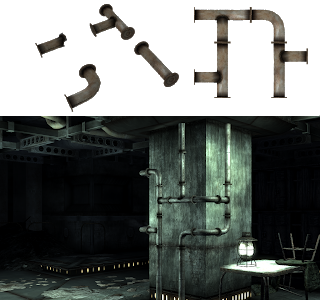
\includegraphics[width=\linewidth]{bilder/pipes}}
  \caption{Beispielhaftes modulares Kit eines Rohr-Systems aus \textit{Fallout 3} (Bethesda Softworks, 2008), \parencite{Burgess}.}
\label{pipes}
\end{figure}
\subsection{Asset}
Die Elemente die ein Kit ausmachen werden \enquote{Assets} genannt und von G. Rehfeld folgendermaßen definiert:
\begin{quote}
\enquote{Assets sind die benötigten Bestandteile eines Spiels. Bei einem Analogspiel die unterschiedlich farbigen Pöppel und Karten, das Spielbrett und die  Würfel. In einem Digitalspiel handelt es sich um alle Objekte, die im Spiel auftauchen: Die Modelle und animierten Figuren, die Spieler und Lebewesen der Welt darstellen, feste Objekte der Spielwelt wie Autos, Bäume, Häuser, Gegenstände wie Waffen, Kleidung etc. Also alles, was man im Film als „Prop“ oder „Requisite“ bezeichnet und dazu dient, die Atmosphäre des Spiels so klar wie möglich darzustellen.} \parencite[S.\,53-54]{rehfeld}
\end{quote}
Nach dieser Definition umfasst \enquote{Asset} viele verschiedene Elemente. In dieser Arbeit wird \enquote{Asset} hauptsächlich für die Bezeichnung fester Objekte in der Spielwelt genutzt und umfasst somit beispielsweise Gebäude, Höhlen oder Raumschiffe.
\subsection{Game-Engine}
Für die Entwicklung von Videospielen werden Game-Engines genutzt. Zu den aktuell bekanntesten gehören Unity und UE \parencite{BestEngine}.
Jeff Ward, Spieleprogrammierer und Dozent, definiert die Leistung und den Nutzen von Game-Engines wie folgt:
  \begin{quote}
  \enquote{...it exists to abstract the (sometime platform-dependent) details of doing common game-related tasks, like rendering, physics, and input, so that developers (artists, designers, scripters and, yes, even other programmers) can focus on the details that make their games unique.
\par
Engines offer reusable components that can be manipulated to bring a game to life. Loading, displaying, and animating models, collision detection between objects, physics, input, graphical user interfaces, and even portions of a game's artificial intelligence can all be components that make up the engine.} \parencite{Engine}
  \end{quote}
Durch Spiele-Engines wird das Entwickeln von Spielen also erheblich erleichtert, da sie viele grundlegende Funktionen bieten und die Komplexität der Spieleentwicklung reduzieren. \parencite{Engine}
\section{Geschichte von Modularität in Videospielen}\label{Geschichte von Modularität }
Ein frühes Beispiel für Modularität in Videospielen ist \textit{Super Mario Bros.} (Nintendo, 1987) für das Nintendo Entertainment System. Die Level des Spiels wurden auf Kästchenpapier entworfen, also auf einem Raster, mit dem die digitalen Koordinaten für das Spiel definiert werden konnten (vgl. Abbildung \ref{marioAnalog}). Nach dem Designprozess wurden die Level von Programmierern Block für Block in das Spiel implementiert \parencite{marioAnalog}.\enlargethispage{10.5pt}
\begin{figure}[H]
\centering
  \makebox[\textwidth]{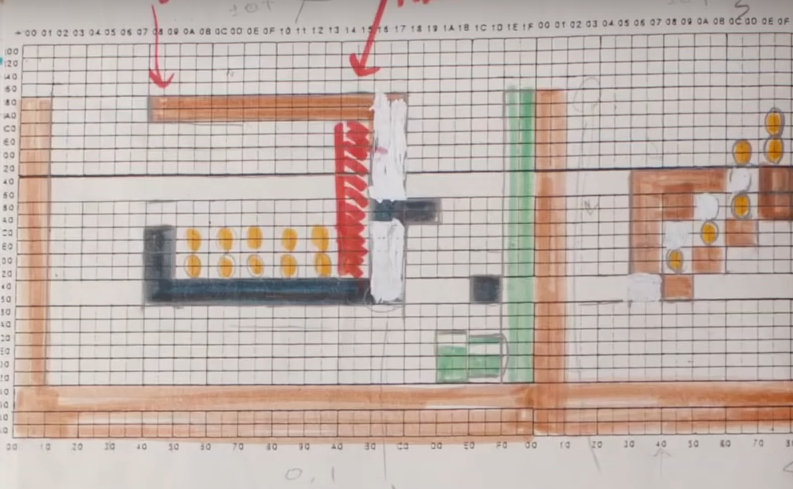
\includegraphics[width=0.8\textwidth]{bilder/marioAnalogAuschschnitt}}
  \caption{Ausschnitt eines Original Entwurfs eines \textit{Super Mario Bros.} Levels. In Anlehnung an \parencite{marioAnalog}.}
\label{marioAnalog}
\end{figure}
\vspace{-14pt}
\enlargethispage{10.5pt}
\begin{figure}[H]
\centering
  \makebox[\textwidth]{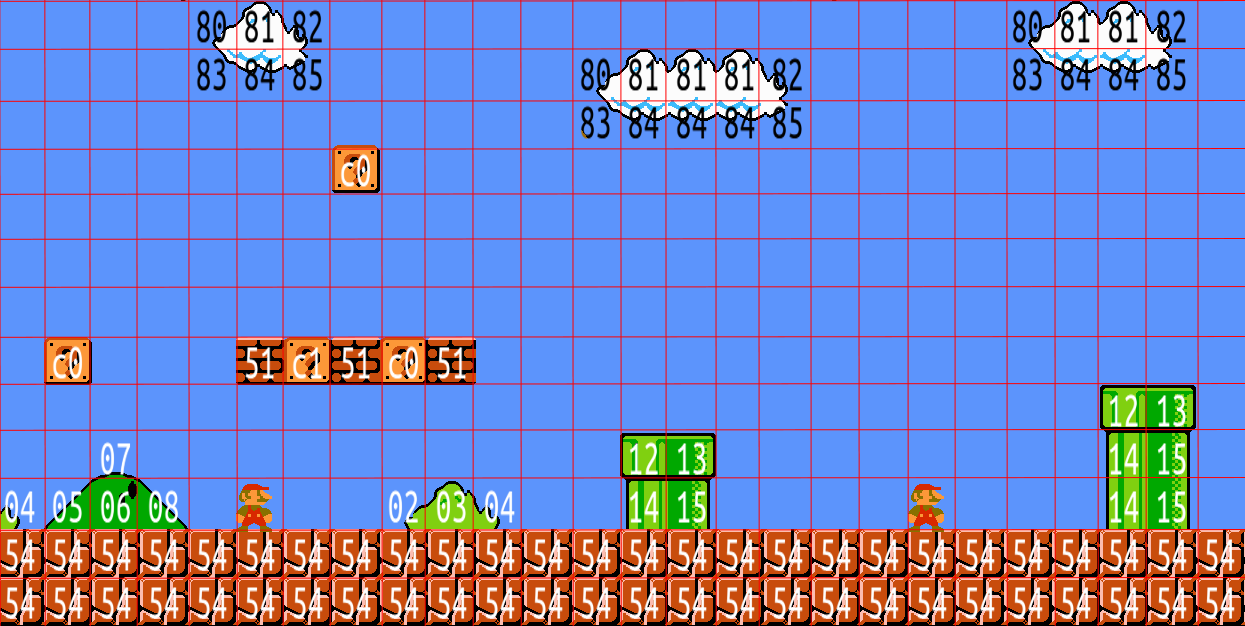
\includegraphics[width=0.94\textwidth]{bilder/SuperMarioBrosAnalysis}}
  \caption{Analyse der Tiles in \textit{Super Mario Bros.}. In Anlehnung an \parencite{MarioTiles}.}
\label{MarioImage}
\end{figure}
\vspace{-10.5pt}
%\begin{figure}[!h]
%\centering
%  \subfloat[][Ausschnitt eines Original Entwurfs eines \textit{Super Mario Bros.} Levels. In Anlehnung an \parencite{marioAnalog}.]{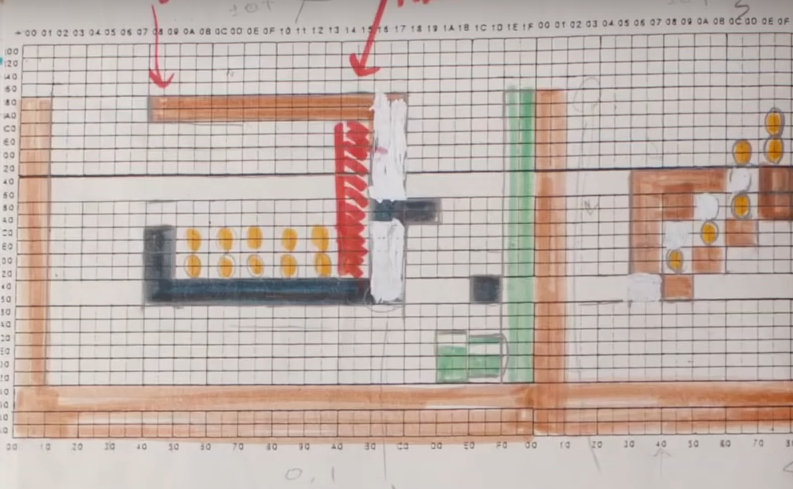
\includegraphics[width=0.42\linewidth]{bilder/marioAnalogAuschschnitt}\label{marioAnalog}}%
%  \qquad
%  \subfloat[][Analyse der Tiles in \textit{Super Mario Bros.}. In Anlehnung an \parencite{MarioTiles}.]{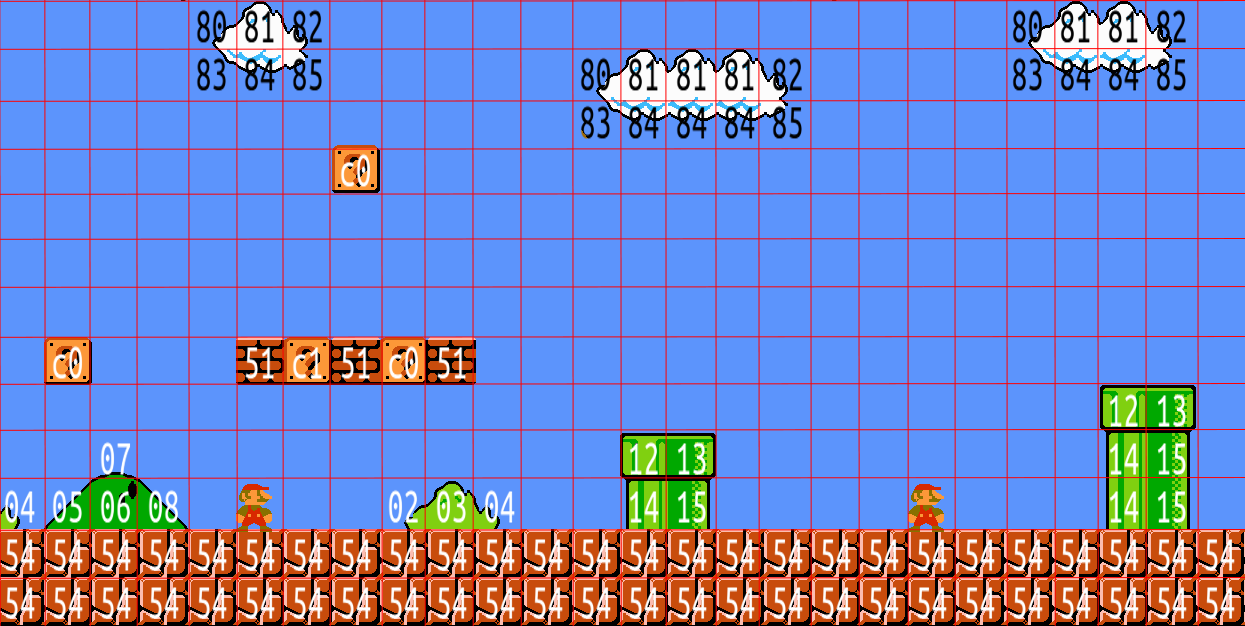
\includegraphics[width=0.52\linewidth]{bilder/SuperMarioBrosAnalysis}\label{MarioImage}}%
%  \caption{Analoges und digitales Level-Layout von Super Mario Bros.}%
%\end{figure}
\par
Alle Elemente der Level wurden mit Hilfe von Tiles\footnote{Ein Tile ist eine Grafik, die mosaikartig zusammengesetzt ein größeres Gesamtbild ergibt.} dargestellt. Wie in der Abbildung \ref{MarioImage} zu sehen, besteht dieser Ausschnitt des Levels aus nur wenigen verschiedenen Tiles. Sie sind in einem Raster angeordnet und wurden so aufgebaut, dass sie nahtlos aneinanderpassen. So ließen sich mit nur wenigen Sprites\footnote{Ein Sprite ist eine zweidimensionale Grafik.} beliebig große Objekte erstellen und ganze Level bauen. Das grüne Rohr kann zum Beispiel mit den Stücken 14 und 15 beliebig verlängert werden. Das gleiche gilt für die Wolken und die Tiles 81 und 84. Diese modulare Herangehensweise erlaubte es den Entwicklern trotz der Hardware-Speicher-Limitierungen von damals größere Level zu entwickeln \parencite{Mario}.
\par
Die fortschreitende Technologie brachte die Möglichkeit mit sich, Spiele im dreidimensionalen Raum zu entwickeln, was als logischen Schluss hatte, dass die meisten Spiele fortan in 3D entwickelt wurden \parencite{GameHistory}. Der Schritt in die dritte Dimension brachte sowohl in der Programmierung als auch beim Design der Spiele neue Hindernisse mit sich, die es zu überwinden galt.
\par
Trotz der fortgeschrittenen Technik waren Speicherplatz und Rechenleistung noch nicht so ausgereift wie heute und stellten weiterhin ein Problem dar, wenn große Welten entwickelt werden sollten. Spiele wie \textit{The Elder Scrolls II: Daggerfall}\footnote{Daggerfall ist ein Open-World-Action-Rollenspiel welches aus der Egoperspektive gespielt wird.} (Bethesda Softworks, 1996) wussten sich durch den Einsatz der Modularität und Prozeduralität zu helfen und umgingen dieses Problem somit \parencite{Fallout4}. Die geschickte Kombination von Modularität und Prozeduralität erlaubte den Entwicklern mit Hilfe weniger modularer Dungeon-Blöcke eine Vielzahl unterschiedlich wirkender Dungeons zu generieren \parencite{Fallout4}. Die algorithmisch erstellten Level sorgten so für sehr viel mehr Abwechslung, wodurch in nur kurzer Zeit etwa 15.000 Orte generiert werden konnten \parencite{Daggerfall}. Die Welt von \textit{Daggerfall} bestand aus zweidimensionalen Sprites, die in einer dreidimensionalen Umgebung platziert wurden. Obwohl diese Technik sich deutlich von der heutigen unterscheidet, ähneln die Modularitätsansätze in \textit{Daggerfall} dennoch denen aktueller Spiele.
\par
\begin{figure}[!h]
\centering
  \subfloat[][Übersicht eines Dungeons aus \textit{Daggerfall}.]{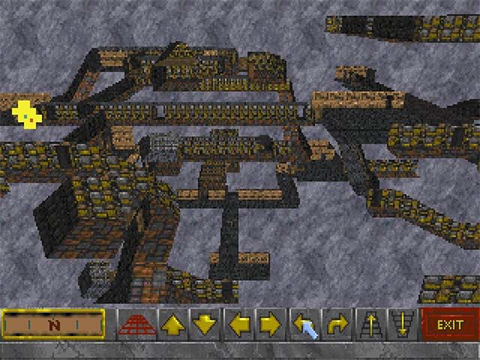
\includegraphics[height=4.4cm]{bilder/Daggerfall}}%
  \qquad
  \subfloat[][Übersicht eines Dungeons aus \textit{Morrowind}.]{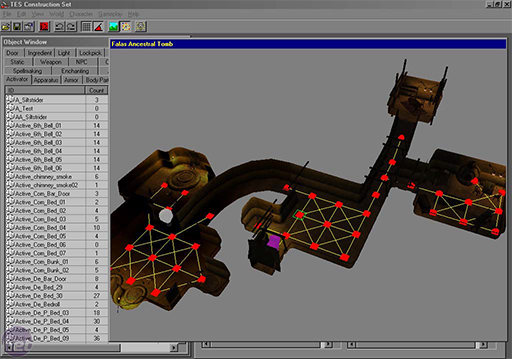
\includegraphics[height=4.4cm]{bilder/Morrowind}}%
  \caption{Beispiele für Modulare Dungeons \parencite{Fallout4P}.}%
\end{figure}
\newpage
\textit{The Elder Scrolls III: Morrowind} (2002) von Bethesda Softworks ist der erste Teil der \textit{Elder Scrolls}-Reihe, der komplett dreidimensionale Assets nutzte und neben der Egoperspektive auch über eine Third-Person-Perspektive verfügte. Auch in diesem Teil wurden die Dungeons mit Hilfe modularer Assets erstellt \parencite{Fallout4}. Dieses Mal wurden sie allerdings nicht prozedural generiert, sondern von Hand erstellt und genau von den Level-Designern geplant. Folglich war die Welt von \textit{Morrowind} kleiner, aber realistischer aufgebaut, als die ihres Vorgängers \parencite{Morrowind}. \textit{Morrowind} hatte nur 0,01 \% der Größe seines Vorgängers \parencite{Daggerfall}, was ein Beispiel für die Möglichkeiten von Modularität und prozeduraler Generierung ist. Ähnlich zu dem System aus \textit{Super Mario Bros.} (Abschnitt \ref{Geschichte von Modularität }) arbeitet der Level-Editor aus \textit{Morrowind} mit einem Raster, auf dem verschiedene modulare Tiles aneinander gesteckt werden können. Dadurch entstehen aus den einzelnen Modulen komplette Höhlensysteme \parencite{Fallout4}.
\par
Der in \textit{Morrowind} genutzte Ansatz wurde auch bei \textit{The Elder Scrolls IV: Oblivion} (Bethesda Softworks, 2006) angewandt. Für einen abwechslungsreicheren Look wurden modulare Assets auch mit vielen individuellen Assets kombiniert. \parencite{Fallout4}
\par
Für \textit{The Elder Scrolls V: Skyrim} (Bethesda Game Studios, 2012) wurde 
das in \textit{Morrowind} und \textit{Oblivion} genutzte System für Modularität weiter verbessert. Zu Beginn der Entwicklung wurden Kits definiert, die jeweils einen Bereich der Spielwelt abdecken sollten. Die Kits beinhalteten Assets, mit denen natürlichere Formen, wie Höhlen und Tunnel, dargestellt werden konnten. Dadurch war es möglich, sich von dem kastenförmigen Erscheinungsbild, welches modulare Ansätze vorher prägte, zu entfernen.
\begin{figure}[H]
\centering
  \makebox[\textwidth]{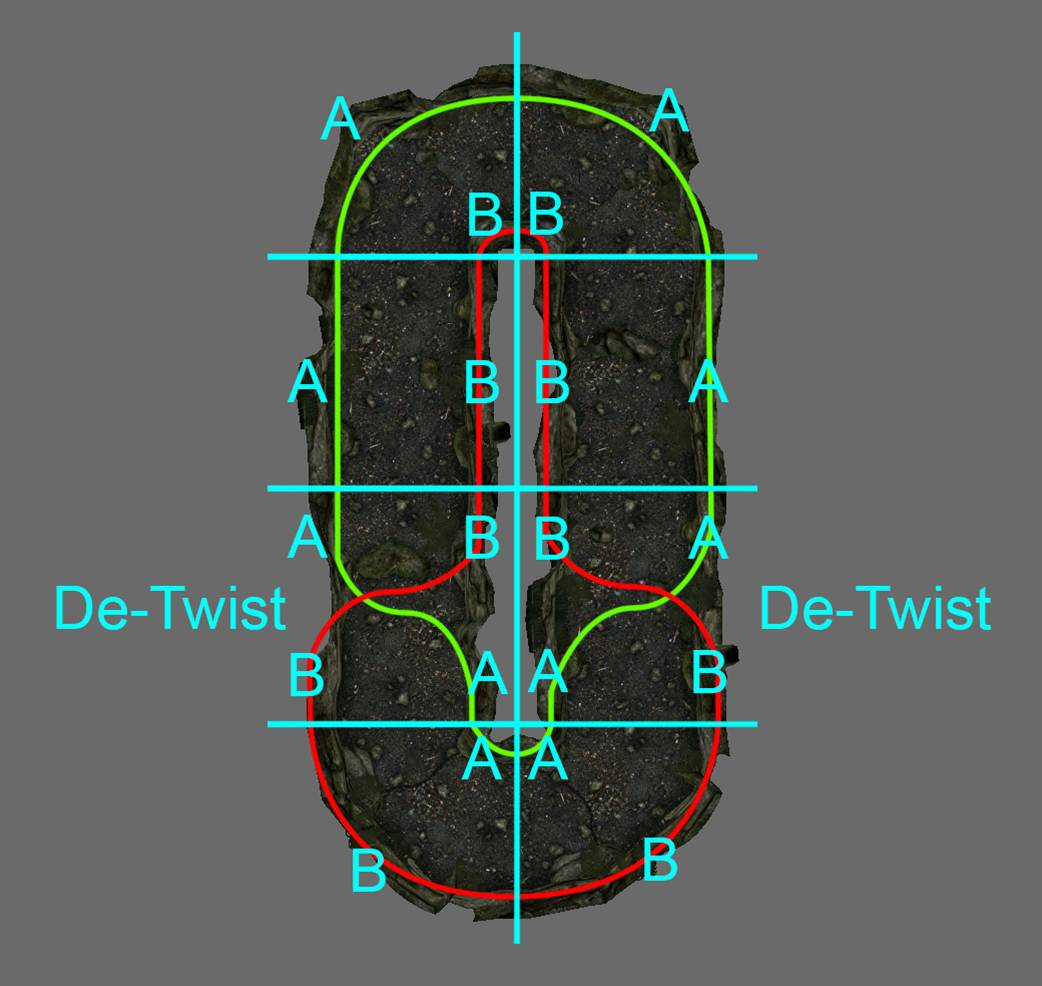
\includegraphics[width=0.6\textwidth]{bilder/asy1}}
  \caption{Asymmetrische Tunnelmodule aus \textit{Skyrim} \parencite{Burgess}.}
\label{ForHonorImage}
\end{figure}
\vspace{-10.5pt}
Hierfür wurden unter anderem asymmetrische Module entwickelt, die sich nur in eine Richtung miteinander verbinden ließen. Die Nutzung asymmetrischer Assets verursacht mehr Arbeit, diese wird aber durch die höhere visuelle Qualität gerechtfertigt. Durch für alle Kits definierte Regeln konnten die Assets der verschiedenen Kits auch gut untereinander kombiniert werden. Dank dieser Technik reichten schon sieben verschiedene Kits, für genügend Abwechslung in den über 400 Leveln \textit{Skyrims}. Bethesdas Hauptziel beim Einsatz von modularem Design war, trotz weniger Mitarbeiter möglichst viele Inhalte generieren zu können. Von den zur Zeit der Entwicklung 90 Mitarbeitern im Entwicklungsteam waren nur zehn für die Level-Erstellung zuständig. \parencite{Burgess}
\par
Mittlerweile ist Modularität eine weit verbreitete Technik in der Videospielindustrie, die je nach spezifischem Einsatzgebiet sehr unterschiedliche Ansätze und Ziele verfolgt. Allen gemeinsam ist die Idee der Wiederverwertung getaner Arbeit, sowie des Einsparens von Speicher und der Optimierung der Performance \parencite{Meler}.
\par
Ein aktuelleres Beispiel für modulares Design in Videospielen ist das Online-Hack-and-Slay \textit{For Honor} (2017) von Ubisoft. In diesem Spiel können sich Spieler mit verschiedenen Kriegern bekämpfen. Diese Kämpfe finden auf verschiedenen, voneinander getrennten Karten, in einem von drei Settings (Ritter, Samurai und Wikinger) statt \parencite{ForHonorMapTypes}.
\par
Für das Entwickeln der Karten werden modulare Kits genutzt. Es gibt Kits, die nur für spezifische Orte auf einer Karte genutzt werden. Die Modularität dieser Kits verliert dadurch an Wert. Ein Vorteil von großer Bedeutung für Ubisoft bleibt aber bestehen: Der Aufbau der Level ist durch ihre Modularität leicht veränderbar. Dies ermöglicht es nach Tests, Gebiete oder einzelne Räume ohne große Umstände für verbessertes Gameplay anzupassen \parencite{ForHonor}. Das ist für ein Kampfspiel, besonders wichtig.
\begin{figure}[H]
\centering
  \makebox[\textwidth]{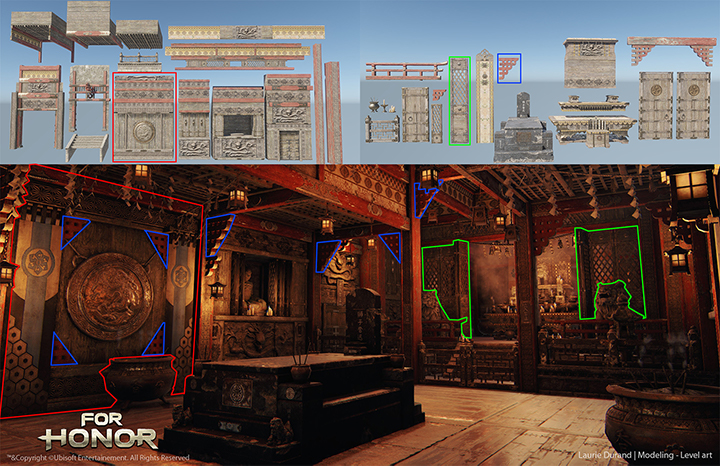
\includegraphics[width=\textwidth]{bilder/ForHonor}}
  \caption{Modulare Assets in \textit{For Honor}. In Anlehnung an \parencite{ForHonor}.}
\label{ForHonorImage}
\end{figure}
\vspace{-10.5pt}
Abbildung \ref{ForHonorImage} zeigt einen Raum, der aus einem solchen Kit entstanden ist. Ergänzend wurde er mit einigen weiteren Assets ausgestaltet. Alle Module in For Honor folgen festen Regeln, die zu Beginn der Entwicklung festgelegt wurden.  Diese Regeln umfassen die genutzte Größeneinheit, unterschiedliche Größen für verschiedene modulare Teile und das Verhalten der Assets auf dem genutzten Raster. \parencite{ForHonor}
\par
Auch viele der nicht modularen Assets in \textit{For Honor} wurden mit Hilfe der Modularität erzeugt. Der Lead-Level-Designer hat zu Beginn des Projektes ein Kit aus Steinen und eines aus Holzbrettern angefertigt. Die anderen 3D-Artists konnten diese Kits nutzen, um die ihnen zugewiesenen Modelle zu erstellen. So konnten die Assets auch bei hoher Entwicklungsgeschwindigkeit mit einem großen Detailgrad entworfen werden. \parencite{ForHonor}
\par
Modularität findet mittlerweile nicht mehr nur für die Gestaltung von Levels Anwendung, sondern auch in anderen Bereichen, wie z. B. der Erstellung von Assets. Wie aufgezeigt wurde, haben sich die dafür genutzten Methoden über die letzten Jahrzehnte durchgehend geändert und verbessert. Die meisten modularen Systeme basieren allerdings immer noch auf der Nutzung von Rastern. Hauptsächlich die Methoden, wie Raster genutzt werden, haben sich weiterentwickelt. Auch aktuell werden immer neue Methoden, beispielsweise die Verwendung künstlicher Intelligenz, in die Produktionsabläufe integriert, die die Vorteile von Modularität weiter ausreizen.
\newpage
\section{Modularität in der Realität}
Nicht nur in Videospielen, sondern auch in der echten Welt werden die Vorteile der Modularität ausgenutzt.
\par
Ein frühes Beispiel für Modularität ist der Gebäudebau. Eines der ersten Systeme welches den modernen Ansätzen ähnelt, wurde ca. 1830 von Henry Manning entwickelt \parencite[Abschnitt 1.1.1]{1837}. Manning verkaufte vorproduzierte Elemente, welche mit einfachen Werkzeugen zu kleinen Häusern zusammengebaut werden konnten \parencite[Abschnitt 1.1.1]{1837}.
\begin{figure}[H]
\centering
  \subfloat[][Ein Gebäude auf Basis eines Grundgerüsts \parencite{geruest}.]{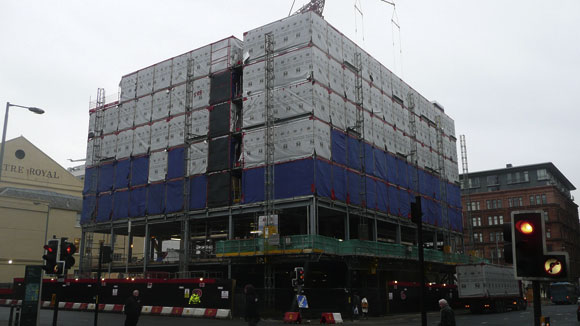
\includegraphics[height=4.3cm]{bilder/geruest}}%
  \qquad
  \subfloat[][Ein Gebäude, dessen Stabilität durch die Wände der Module entsteht \parencite{wand}.]{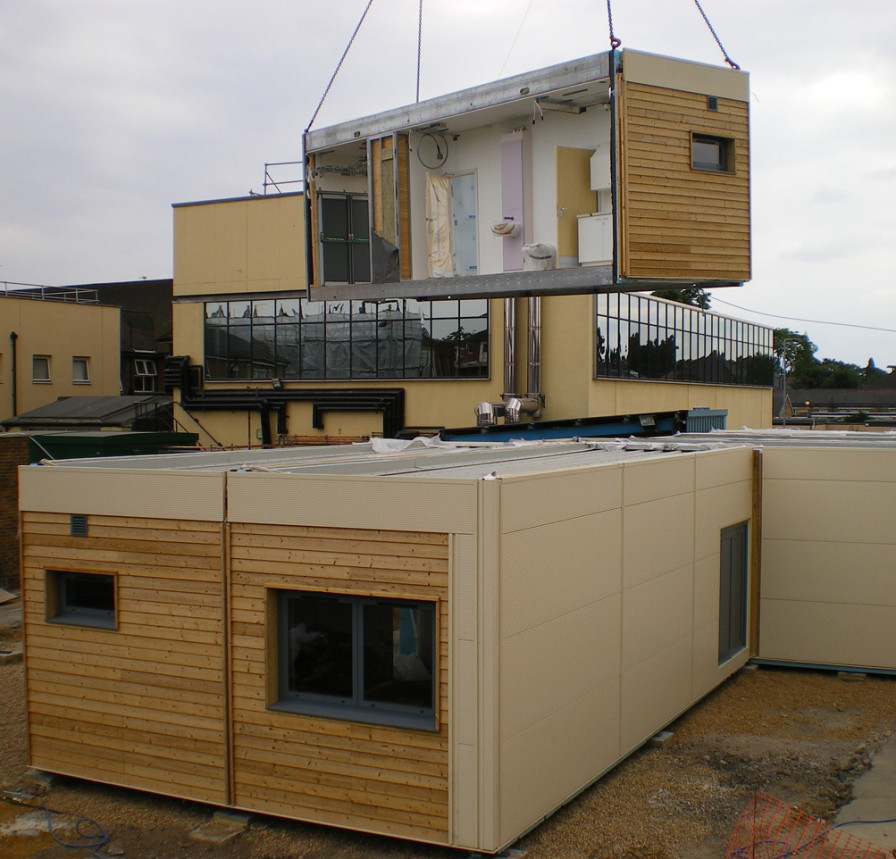
\includegraphics[height=4.3cm]{bilder/Wand}}%
  \caption{Beispiele der zwei genannten Methoden für den Bau modularer Gebäude.}%
\end{figure}
\vspace{-10.5pt}
Heutzutage werden für den Bau modularer Gebäude hauptsächlich zwei verschiedene Methoden genutzt. Erstere findet vor allem bei größeren Bauwerken Verwendung. Hier wird zuerst ein Grundgerüst gebaut, in das die Module eingesetzt werden. Die Lastverteilung verläuft hier über Eckpfeiler. Die andere Methode arbeitet mit Modulen, deren Lasten über die Wände verteilt werden. Letztere kann nur eine Höhe von 4 bis 8 Stockwerken erreichen. \parencite{Lawson}
\par
Der Produktionsablauf unterscheidet sich in vielen Punkten von der normalen Art Gebäude zu errichten, bei welcher der Großteil der Arbeit vor Ort auf der Baustelle durchgeführt wird. Die genutzten Module werden in einer Fabrik, abseits der Baustelle, angefertigt und dann vor Ort mit dem  Fundament und anderen nicht-modularen Bauelementen verbunden. So ist es (gegenüber der herkömmlichen Methode) möglich, die Bauzeit um bis zu 50\%  zu verkürzen. So können die neuen Räumlichkeiten schneller genutzt werden und das Umfeld der Baustelle wird nicht so lange belastet, wie es normalerweise der Fall ist. \parencite{Lawson}
\par
Mit der Anzahl wiederverwendeter Module sinken die Kosten, weil das Modul nur einmal entworfen werden muss und dann immer wieder auf die gleiche Art produziert werden kann \parencite{Lawson}. Dieser Vorteil gleicht der Wiederverwendbarkeit der Module in Videospielen, die ebenfalls nur einmal designt und dann beliebig oft eingesetzt werden können.
\par
Das wohl offensichtlichste Beispiel sind LEGO-Steine. LEGO hat ein System entwickelt bei dem sich fast alle der verschiedenen produzierten Teile miteinander kombinieren lassen und das auf viele verschiedene Arten. Sechs gleichfarbige Sechser-Blöcke können auf 915.103.765 Arten \parencite[S.\,10]{LegoBuch} verbunden werden, um verschiedene Formen darzustellen. Auch die Teile der LEGO-Figuren lassen sich beliebig miteinander kombinieren. 
\par
Es existieren LEGO-Sets, die standardmäßig darauf ausgelegt sind, dass drei unterschiedliche Modelle, aus den im Set vorhandenen Teilen, gebaut werden können. Zusätzlich lassen sich, wie bei allen LEGO-Sets, noch weitere Modelle bauen, die nicht durch die Anleitung vorgegeben sind \parencite{Lego3in1}. Seit 2007 gibt es modulare Sets, die diesen Ansatz weiter verfolgen, in denen zusammengebaute kleinere Teile auf verschiedene Weisen miteinander verbunden werden können um das Aussehen des Modells auf einfache Art abzuwandeln \parencite{LegoMod}.
\begin{figure}[H]
\centering
  \makebox[\textwidth]{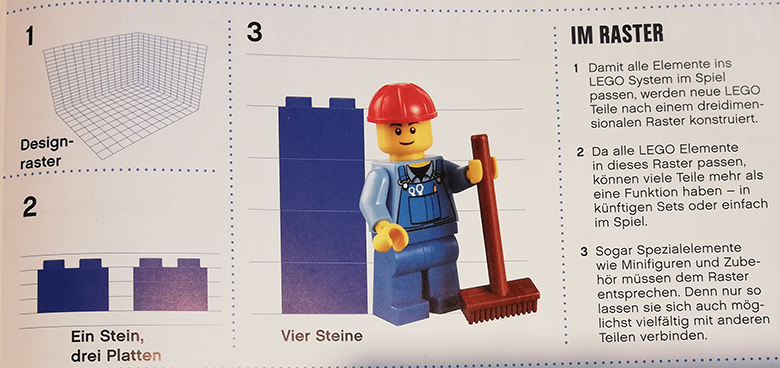
\includegraphics[width=\textwidth]{bilder/legoRaster}}
  \caption{Das Raster nach dem alle LEGO-Steine Entwickelt werden. In Anlehnung an \parencite[S.\,11]{LegoBuch}.}
\label{legoRaster}
\end{figure}
\vspace{-10.5pt}
Der modulare Ansatz ermöglicht es dem Unternehmen neue Sets zu entwerfen, die zum Beispiel den Eiffelturm darstellen, ohne dass dafür neue Teile entwickelt werden müssen. Stattdessen kann auf die bestehende Palette von LEGO-Steinen zurückgegriffen werden. Damit dies funktioniert, müssen alle Steine Regeln befolgen und auf einem bestimmten Raster entworfen werden (vgl. Abbildung \ref{legoRaster}). Hierdurch sind alle jemals entwickelten Teile zumindest stückweise miteinander kompatibel \parencite[S.\,11]{LegoBuch}.
\par
Es existieren viele weitere Anwendungsgebiete für Modularität. Die hier aufgezeigten Beispiele sollen genügen, um einen Eindruck zu vermitteln, welche Möglichkeiten und Vorteile Modularität mit sich bringen kann.
\chapter{Grundlagen der Asset-Erstellung}
In diesem Kapitel wird auf die grundlegenden Vorgehensweisen für die Erstellung und Implementierung von 3D-Modellen für Videospiele eingegangen. Da die Vorstellung aller Workflows rund um die Erstellung dreidimensionaler Modelle den Rahmen dieser Arbeit übersteigt, konzentriert sich der nachfolgende Abschnitt lediglich auf den traditionellen Ansatz.
\section{Planung}
Der erste Schritt in der Entwicklung eines Assets ist die Planung. Die Länge dieser Phase ist abhängig vom jeweiligen Projekt und dessen Fortschritt. Sind der Stil und das Setting des Spiels noch nicht definiert, wird diese Phase mehr Zeit in Anspruch nehmen.
\par
Entscheidend sind auch die Komplexität des Assets und sein geplanter Nutzen. Handelt es sich zum Beispiel um ein Fahrzeug, das der Spieler benutzen soll, müssen vorab Regeln definiert werden, die das Modell erfüllen muss, um mit der Spielfigur und der Umwelt kompatibel zu sein. Dazu gehören das Zusammenspiel mit der Spielphysik und die Beeinflussung durch die Programmierung. Für Gebäude sollte zum Beispiel die Größe der Spielfigur für Türen und Abstände in den Räumen beachtet werden. Um Problemen mit der Kamera vorzubeugen, sollte das Verhalten der Kamera bei der Planung von Decken und Wänden bedacht werden. Jedes Modell-, beziehungsweise jeder Modell-Typ, bedarf spezifischer Planung, damit es im Spiel ordnungsgemäß funktioniert. Um große Überarbeitungen in späteren Revisionen des Modells zu verhindern, sollte bereits zu Beginn sichergestellt werden, dass das geplante Modell die Regeln des Projektes einhält.
\par
Um die Umsetzung des Assets zu beschleunigen und möglichst wenig Iterationsschritte zu benötigen, sollte vor der eigentlichen Modellierungsphase ein oder mehrere Konzeptgrafiken oder wenigstens andere Referenzgrafiken vorliegen.
\newpage
\section{Modellierung}
In diesem Abschnitt werden der Aufbau eines 3D-Modells und die Arbeitsschritte in seinem Produktionsablauf erklärt. Der Abschnitt basiert im wesentlichen auf dem Handbuch von T. Beck \parencite{blender} und fasst die hier relevanten Aspekte zusammen. Bei der vorgestellten Methodik wird erst das Modell erzeugt und danach eine passende Textur generiert. Es ist auch möglich, diese Schritte zu vertauschen und Modelle von einer Textur ausgehend zu erzeugen. Auf dieses Verfahren wird hier aber nicht eingegangen\footnote{Der interessierte Leser findet hierfür ein Beispiel in dem \enquote{Modular Building Breakdown} von Jacob Norris \parencite{Norris}.}. 
\par\textbf{Grundlagen und Begriffe}
\par
Grundlegend bestehen 3D-Modelle aus einer Ansammlung von Punkten in einem dreidimensionalen Raum. Diese Punkte heißen Vertex (Singular), bzw. Vertices (Plural). Eine Verbindung zwischen Zweier dieser Punkte heißt Kante oder Edge. Bilden mehrere Edges eine geschlossene Fläche, so spricht man von einem Face.
\begin{figure}[H]
\centering
  \makebox[\textwidth]{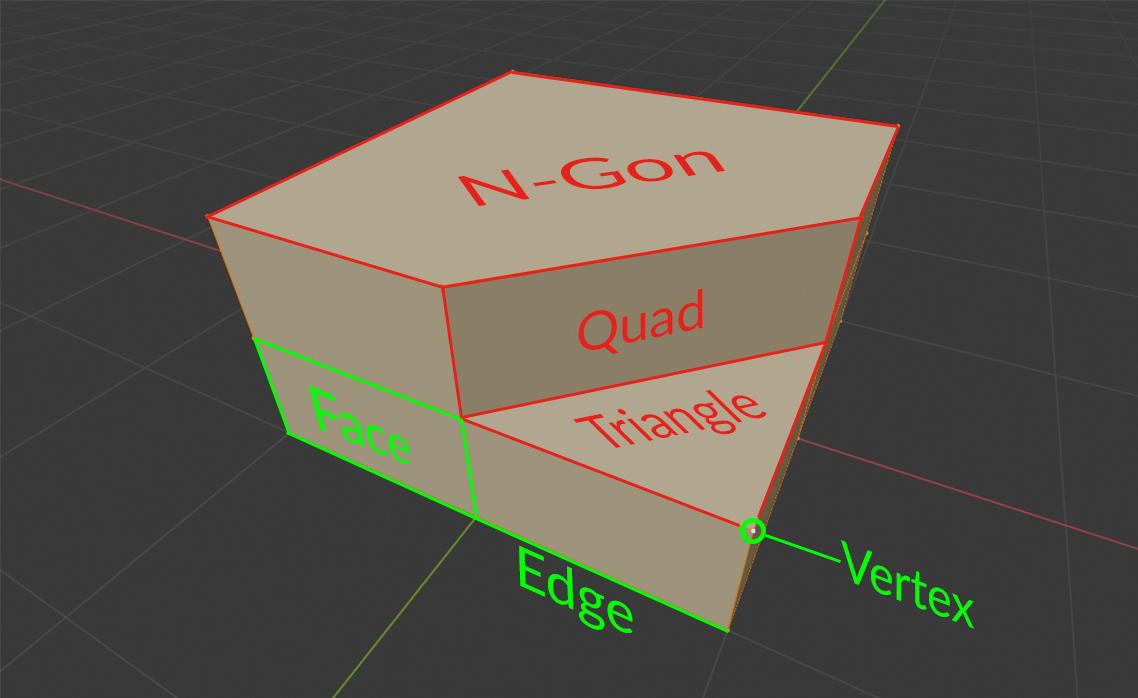
\includegraphics[width=0.9\textwidth]{bilder/BlenderCube}}
  \caption{Darstellung der Bestandteile eines Meshes.}
\label{BlenderCube}
\end{figure}
\vspace{-10.5pt}
Wie in Abbildung \ref{BlenderCube} ersichtlich, kann die Anzahl der verwendeten Vertices zur Bildung eines Faces variieren. Man unterscheidet in der Regel zwischen Triangles (Face mit drei Vertices), Quads (Face mit vier Vertices) und N-Gons (Face mit fünf oder mehr Vertices). Im Hintergrund bestehen alle Flächen aus Dreiecken, egal, wie viele Eckpunkte sie haben \parencite[S.\,82-83]{blender}. Während des Modellierens ist es von Vorteil mit Quads zu arbeiten, sie lassen sich leichter unterteilen und wieder zu einem großen Quad zusammenführen. N-Gons sollten vermieden werden, weil diese zu Fehlern in der Darstellung und Manipulation führen können.
\par
Während Vertices und Edges die Form eines Modells definieren, repräsentieren Faces die sichtbaren Flächen des Objekts. Die Richtung, aus der eine Fläche zu sehen ist, ist abhängig von ihrer Flächennormalen. Wenn die Flächennormale nicht manipuliert wurde steht sie senkrecht auf der zugehörigen Fläche \parencite[S.88]{blender}.
\enlargethispage{14pt}
\newpage
Von der der Flächennormalen abgewendeten Seite aus ist die Fläche unsichtbar. Es gibt in den meisten Engines eine Funktion für beidseitiges Rendern von Faces, dies ist aber sehr Performanceintensiv.
\par
Das sogenannte Shading bestimmt das Erscheinungsbild eines Meshes. Zwei spezielle Formen die direkt mit der Topologie des Models arbeiten, sind Flat und Smooth Shading.
\par
Bei der normalen Darstellung (Flat) wird jedes Face für sich gerendert, ohne die angrenzenden Faces zu beachten. Für Smooth Shading wird zwischen den Flächennormalen interpoliert, wodurch eine glattere/weichere Erscheinung des Meshes entsteht. Diese beiden Modi können auf einzelne Faces oder das gesamte Mesh angewendet werden. Dadurch sind sowohl weiche als auch harte Flächen auf einem Objekt darstellbar. \parencite[S.\,388-394]{blender}
\par
Nach den Grundlagen folgt jetzt der eigentliche Prozess der Modell-Erstellung.
\par
\textbf{Prozess der Modell-Erstellung}
\par
Für die Modell-Erstellung kommen nun die Konzeptgrafiken und Referenzen zum Einsatz. Gute Konzepte können als Blaupause im 3D-Tool genutzt werden, wodurch das Konzept detailgetreu nachgebildet werden kann. Auch Referenzen eignen sich, wie bereits erwähnt, um das Modell nachzubauen.
\par
Durch Manipulation der Vertices, Edges und Faces kann jede mögliche Form modelliert werden. In der Videospielproduktion wird häufig auf Low-Poly-Modelle zurückgegriffen. Das heißt, dass bei der Modellierung die Anzahl der Polygone, so gering wie möglich gehalten werden. Hierdurch verlieren die Modelle zwar an Detail, die Darstellungsgeschwindigkeit wird aber erhöht. Die fehlenden Details können teilweise im Nachhinein mit Hilfe einer Normal-Map (siehe Abschnitt \ref{Texturierung1}) ausgeglichen werden.
\par
Auch für den nächsten Arbeitsschritt hat der 3D-Artist zwei Möglichkeiten. Entweder wird zuerst das Low-Poly-Modell erstellt und aus einer Kopie dessen dann ein High-Poly-Modell, oder es wird direkt das High-Poly-Modell erstellt. Ein High-Poly-Modell ist ein Asset mit einer hohen Auflösung, in Bezug auf die genutzten Triangles. Bei letzterer Variante wird im Nachhinein durch Retopologie ein Low-Poly-Modell erzeugt.
\par
In dieser Arbeit wird der erste Ablauf zur Erstellung der 3D-Modelle genutzt.
\par
Es empfiehlt sich, die gewünschten Formen zuerst mit primitiven Objekten nachzubilden, die dann z. B. durch Unterteilen, Auftrennen, Zusammenfügen und Verformen\footnote{Dies ist nur eine Auswahl der Möglichkeiten, die zur Manipulation von Meshes zur verfügen stehen. Eine ausführliche Liste bietet das Blender Manual \parencite{blendermanual} im Kapitel Mesh Editing.} so angepasst werden können, dass das Modell den Vorgaben entspricht. Die Möglichkeiten der Mesh-Bearbeitung hängen vom genutzten 3D-Tool ab, aber alle Tools decken prinzipiell die gleichen Funktionen ab.
\newpage
In wie weit die Details der Vorgaben nachgebildet werden, hängt vom Stil, den Fähigkeiten des 3D-Artist und dem Budget\footnote{Das \enquote{Budget} bezeichnet die Menge an Ressourcen, die ein Objekt oder eine Szene verbrauchen darf, ohne dass die Performance des Spiels ungewollt beeinflusst wird.} des Models ab.
\par
Mit der Low-Poly Variante können schon erste Tests in der Engine durchgeführt werden, wie beispielsweise die Überprüfung der Vorgaben und Regeln des Projektes. Funktioniert das Modell wie geplant, kann eine Kopie, die als Basis der High-Poly-Variante dient, angelegt werden. Funktionen und Tools wie der Remesh Modifier aus Blender (vgl. Abbildung \ref{remesh}) können gleichmäßige Verteilungen von Flächen in Meshes erzeugen. Diese Gleichmäßige Verteilung ist wichtig um beim sogenannten Sculpting und auch sonstigen weiteren Anpassungen des Meshes einen konstanten Detailgrad zu erhalten \parencite{Grabstein}.
\begin{figure}[H]
\centering
  \makebox[\textwidth]{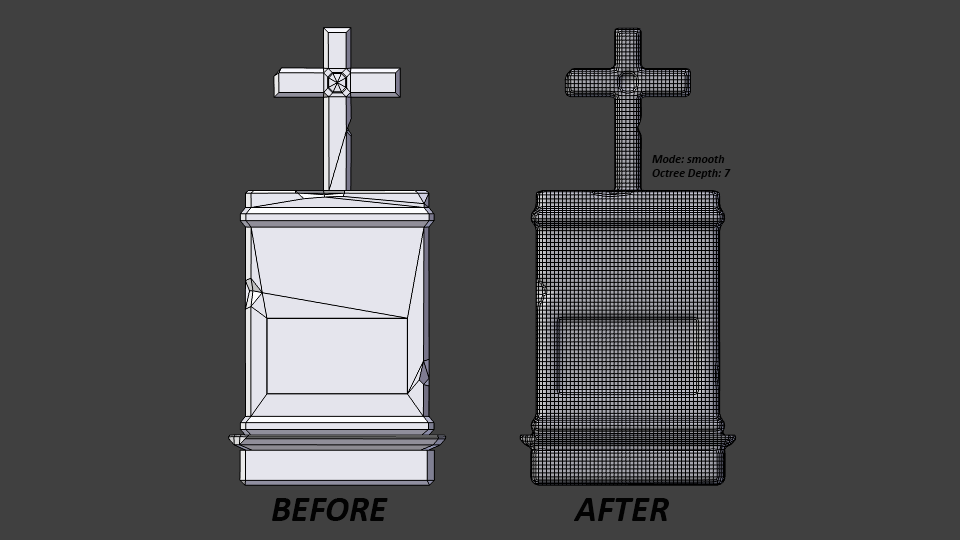
\includegraphics[width=0.7\textwidth]{bilder/remesh}}
  \caption{Ein Grabstein vor und nach dem Anwenden des Blender Remesh Modifierers \parencite{Grabstein}.}
\label{remesh}
\end{figure}
Neben der Technik das ganze Mesh so oft zu unterteilen, bis es den gewünschten Detailgrad abbilden kann, ist es auch möglich mit dynamischer Topologie zu arbeiten. Bei diesem Verfahren wird nur an den modifizierten Stellen des Objekts neue Topologie erschaffen. So kann die Anzahl der Triangles des Meshes relativ gering gehalten werden.
\par
Unabhängig von der gewählten Methode kann das Mesh anschliessend, wie Ton bearbeitet werden. Dies ermöglicht organische und detailreiche Modelle \parencite[S.\,172-189]{blender}.
\subsection{Texturierung}\label{Texturierung1}
In diesem Abschnitt wird auf Möglichkeiten eingegangen das äußere Erscheinungsbild eines Models zu verändern. Dies ist mit Hilfe von Texturen und Materialien möglich. Es werden verschiedene Arten von Texturen und ihr Einfluss auf Modelle erläutert.
\par
Die Darstellung des Models ist abhängig von dem oder den zugewiesenen Materialien. Materialien (englisch Materials) sind in allen 3D-Tools und Engines verschieden aufgebaut, funktionieren im Prinzip aber gleich. Es gibt Slots, die mit verschiedenen Texturen gefüllt werden können, und Parameter, mit denen die Erscheinung des Materials weiter beeinflusst werden kann.
\newpage
Neben den \enquote{normalen} Materialien existieren Physically Based Rendering (PBR) beziehungsweise Physically Based Shading (PBS) Materialien, der Einfachheit halber wird ab hier PBR als Überbegriff genutzt. PBR-Materialien erlauben es, annähernd physikalisch korrekte Oberflächen darzustellen. Hierfür werden Texturen mit Messwerten echter Materialien benötigt \parencite[S.\,490-492]{blender}. Dies verringert die für die Material-Erstellung benötigte Zeit, weil mögliche schrittweise Annäherung entfallen \parencite[S.\,490-492]{blender}. Des Weiteren sind PBR-Systeme in allen PBR unterstützenden 3D-Anwendungen ähnlich aufgebaut, wodurch sie unabhängig von der Anwendung gleich aussehen, ohne einer speziellen Konfiguration zu bedürfen \parencite[S.\,490-492]{blender}.  
\par
Im Folgenden werden die geläufigsten Texturen aufgelistet und ihre Funktion erklärt.\footnote{Eine Übersicht mit Beispielen und weiteren Maps ist auf dem Youtube Kanal von FlippedNormals, in dem Video Texture Maps Explained \parencite{flipped}, zu finden.} Zudem wird darauf eingegangen, ob es bei der jeweiligen Textur Unterschiede für PBR und nicht PBR gibt.
\begin{description}
	\item[Diffuse / Albedo Map]~\par
	Die Diffuse, (bzw. bei PBR-Materialien Albedo) Map, sorgt für die grundlegende Farbe des Modells. Für nicht PBR Materials sind in dieser Textur neben der Farbe auch Schattierungen und Ambient Occlusion enthalten \parencite[S.\,495]{blender}. Ambient Occlusion oder Umgebungsverdeckung erzeugt an Kanten und anderen Flächen mit geringem Abstand Verdunkelungen. Dies beruht auf dem Prinzip, dass weniger Licht an Orte gelangt, die wenig Platz für Streuung zulassen \parencite[S.\,362]{blender}. Diese Texturen können durch direktes Zeichnen auf dem Modell in einem 3D-Tool oder in einem externen Grafikprogramm wie \textit{Adobe Photoshop} angefertigt werden.
	\item[Normal Map]~\par
	Enthält ein Material Normal Maps, kann die äußere Erscheinung des Models verändert werden, ohne seine Geometrie anzupassen. So ist es möglich, Low-Poly-Modelle hochwertiger und teilweise sogar wie High-Poly-Modelle aussehen zu lassen. Die Normal Map manipuliert die Ausrichtung der Normals auf den Faces und kann so beliebige Oberflächenstrukturen vortäuschen, auch wenn das Modell eine glatte Oberfläche besitzt. Jeder Pixel der Map repräsentiert einen, über einen RGB-Wert definierten Richtungsvektor, der mit den bestehenden Normals des Models verrechnet wird. Durch diese Manipulation wird die Interaktion von Licht und Schatten mit der Oberfläche des Objektes verändert. \parencite[S.\,421-422]{blender}
	\item[Bump Map]~\par
	Bump Maps ähneln in ihrer Funktion den Normal Maps. Auch sie ändern das Erscheinungsbild des Models, ohne die Geometrie zu verändern. Der Effekt wird bei Bump Maps durch Graustufen erreicht. Schwarz stellt eine maximale Vertiefung und Weiß eine maximaler Erhöung dar, 50-prozentiges Grau lässt die Oberfläche unverändert. \parencite[S.\,420-421]{blender}
	\newpage
	\item[Displacement Map]~\par
	Das letzte Beispiel für Texturen, welche die Form der Models verändern, ist die Displacement Map. Diese verändert im Gegensatz zu den vorherigen Maps wirklich die eigentliche Geometrie des unterliegenden Objektes. Sie arbeitet wie die Bump Map mit Graustufen, Weiß führt zu einer maximalen Erhöhung und Schwarz zu einer maximalen Vertiefung, 50-prozentiges Grau steht wieder für keine Veränderung. Für eine akkurate Abbildung der Details aus der Textur benötigt das Mesh eine hohe Auflösung, folglich ist diese Methode für Spiele eher ungeeignet. Sie wird hauptsächlich für den Erstellungsprozess genutzt, um dem Modell weitere Details hinzuzufügen, die später in eine Normal Map übertragen werden. \parencite[S.\,422-423]{blender}
	\item[Specular Map]~\par
	Specular Maps werden für nicht PBR-Materialien genutzt, um zu definieren, an welchen Stellen das Modell Glanzpunkte erzeugen kann. Auch die Specular Map ist in Graustufen aufgebaut. Die Stärke des Glanzes wird durch den Grauwert bestimmt: schwarze Stellen glänzen gar nicht und weiße am stärksten. \parencite[S.\,423]{blender}
	\par
	Für PBR-Materialien werden Specular Maps nur in Sonderfällen genutzt. Eis, Wasser und Haut sind Beispiele hierfür. Die Map wird hier genutzt, um die richtige Lichtbrechung zu definieren \parencite{Jess}
	\item[Roughness / Gloss Map]~\par
	Für PBR-Materialien werden Roughness  Maps genutzt, um raue und glatte Bereiche auf einem Modell zu erzeugen. Roughness und Gloss Maps sind im Prinzip das Gleiche, aber die Auswertung des Helligkeitswerts der Textur ist invertiert. Bei einer Gloss Map repräsentiert ein heller Pixel eine sehr glatte Fläche, bei einer Roughness Map wäre die Fläche sehr rau und würde nur wenig bis keine Reflexion erzeugen. \parencite[S.\,496-497]{blender}
\end{description}
Texturen können nur auf ein Modell angewendet werden, wenn dieses entsprechend vorbereitet wurde. Dafür muss es den Prozess des UV-Unwrappings durchlaufen. Hier wird das Mesh aufgetrennt und auf eine zweidimensionale Fläche ausgebreitet. In den meisten 3D-Tools gibt es mehrere Möglichkeiten, das Mesh automatisch aufzutrennen, in der Regel ist es aber besser, diesen Vorgang manuell durchzuführen. Hierfür werden die Edges, an denen das Modell zerschnitten werden soll, markiert und im Anschluss der Unwrap-Vorgang gestartet, der das UV-Layout erzeugt. Über das UV-Layout wird definiert, welcher Ausschnitt einer Textur auf welcher Fläche des Meshes abgebildet wird. \parencite[S.\,445-455]{blender}
\par
Texturen wie die Normal Map können \enquote{gebacken} werden. Für diesen Vorgang werden eine High- und eine Low-Poly Version des gleichen Models benötigt \parencite[S.\,422]{blender}. Die Low-Poly- Version auf welche die Details des High-Poly-Meshes gebacken werden, muss unwrapped sein, damit die Details auf eine 2D-Ebene projiziert werden können \parencite[S.\,513-518]{blender}. Während des \enquote{Backens} werden die Oberflächennormalen des High-Poly-Models in die zugehörigen RGB-Werte übersetzt und in einer Normal Map gespeichert \parencite[S.\,422]{blender}.
\enlargethispage{10.5pt}
\par
Für Spiele wie zum Beispiel \textit{World of Warcraft} (Blizzard Entertainment, 2004) werden nur Low-Poly- Modelle mit Diffuse Texturen genutzt, die nur die Farbe des Modells enthalten \parencite{WoW}. Für die Erstellung dieser Texturen werden High-Poly-Meshes genutzt, deren Details dann auf verschiedene Texturen gebacken werden und anschließend in einer Diffuse Map zusammen geführt werden \parencite{WoW}. Mit dieser Methode wird ein spezieller Look erzeugt und die Speichernutzung reduziert.
\par
Mit den sogenannten 3D-Zeichenprogrammen, wie beispielsweise \textit{Substance Painter} , können Materialien mit allen benötigten Texturen auf 3D Modelle angewendet werden. So können bestehende Materialien manipuliert oder neue angelegt werden. Die Materialien können auf die Beschaffenheiten des Modells eingehen und zum Beispiel Verschleiß an Kanten simulieren. So können in kurzer Zeit detailreiche, realistische Materialien erzeugt werden.
\par
Alle Materialien müssen vor dem Export aus dem 3D-Tool allen zugehörigen Faces des Objekts zugewiesen sein und die Quads des Models sollten in Triangles übersetzt werden (\enquote{Triangulation}). Game-Engines arbeiten nur mit Triangles und übersetzen das Modell selber in Triangles wenn es aus Quads und N-Gons besteht. Bei diesem Vorgang kann es zu Fehlern mit den Flächennormalen kommen. Wird die Triangulation vor dem Export durchgeführt, sind diese Fehler vermeidbar.
\section{Implementierung}\label{Implementierung1}
Für die Erstellung eines Videospiels mit den angefertigten Assets wird eine Game-Engine wie z. B. UE benötigt. Für ein performantes Spiel und eine fehlerfreie Darstellung müssen tiefgreifende Aspekte der Engine verstanden werden. Daher wird im Folgenden auf die Funktionsweise von Realtime Rendering eingegangen, welches für die Darstellung in Spielen genutzt wird.
\par
Alle in der Engine verwendeten Modelle werden in einen Verbund aus Dreiecken übersetzt, weil Grafikkarten (GPUs) mit Dreiecken rechnen \parencite{gpu}. Jedes Mesh wird in der Game Engine in zwei Teilen abgespeichert, dem Vertex Buffer und dem Index Buffer \parencite{gpu}. Der Vertex Buffer enthält eine Liste aller Vertices des Meshes \parencite{gpu}. Dazu gehören Position des Vertex, UV-Koordinaten, Ausrichtung der Normals und weitere \parencite{gpu}. Der Index Buffer enthält Informationen darüber, welche Vertices miteinander Dreiecke bilden und so das Mesh formen \parencite{gpu}. Zusätzlich zu dem Index und Vertex Buffer werden dem Mesh ein oder mehrere Materialien zugewiesen \parencite{gpu}. 
\par
Die Materialien werden in der Engine selbst erstellt und mit den vorgesehenen Texturen konfiguriert. Sie können nicht aus den 3D-Tools, mit denen das Mesh erstellt wurde, übernommen werden. Die Material-Systeme der Engines und die der 3D-Tools sind in der Regel nicht kompatibel.
\newpage
Für die Darstellung des Meshes auf dem Bildschirm wird für jeden Frame eine Folge von Schritten durchlaufen, die sich wie folgt zusammenfassen lassen:
\begin{enumerate}
\item Im ersten Schritt, dem \textit{Input Assembly}, werden anhand des Index Buffers die Vertices aus dem Vertex Buffer miteinander zu Dreiecken verbunden.
\item Dann findet das \textit{Vertex Shading} statt, bei dem die aktuelle Ausrichtung und Position des Meshes in Relation zur Kamera mit allen Vertices verrechnet wird. So wird die Gesamtansicht bestimmt und welche Teile des Objektes zu sehen sind.
\item Die \textit{Rasterization} erzeugt aus jedem Triangle eine gerasterte Fläche, über die die Vertex-Normalen, UV-Koordinaten und weitere Eigenschaften der Vertices interpoliert werden.
\item Der Schritt des \textit{Pixel Shading} ordnet jedem Pixel in der gerasterten Fläche abhängig von Material, Licht und anderen Einflüssen eine Farbe zu.
\item  Zuletzt wird \textit{Render Target Output} durchgeführt, um die berechneten Werte für die Darstellung weiterzuleiten. Es gibt einen Zwischenschritt, der überprüft, ob die errechneten Pixel angezeigt werden sollen. Es wird unter anderem überprüft, ob Pixel nicht sichtbar sind, weil das zugehörige Objekt von einem anderen Objekt verdeckt wird oder ob ein Pixel durchsichtig ist. Dann wird der dahinterliegende Pixel genutzt.
\vspace{-10.5pt}
\begin{flushright}\parencite{gpu}\end{flushright}
\end{enumerate}
Das Rendering ist damit abgeschlossen.
\par
Die Grafikkarte wird bei der Bearbeitung von Bildern von der CPU unterstützt. Diese sendet Draw Calls an die Grafikkarte und übergibt der Grafikkarte die benötigten Daten, um die Draw Calls auszuführen. Ein Draw Call enthält Information über das zu rendernde Mesh, sein Material und seine sonstigen Eigenschaften. Jeder Draw Call wird vom Grafikkarten-Treiber übersetzt und auf Fehler überprüft. Dadurch entstehen für jeden Draw Call Grundkosten, die sich in verbrauchter Zeit widerspiegeln. Für jedes Material wird ein eigener Draw Call abgesetzt; das heißt, wenn ein Mesh mit drei Materials ausgestattet ist, löst es auch drei Draw Calls aus.
\par
Weil die Grafikkarte von der CPU abhängig ist und die CPU jeden Draw Call durcharbeiten muss, haben diese einen direkten Einfluss auf die Framerate. Die Anzahl an Draw Calls sollte folglich gering gehalten werden. \parencite{gpu}
\par
In der Engine kann der Aufbau eines Objektes nicht geändert werden, lediglich Skalierung und Rotation können angepasst werden. Das hat aber keinen Einfluss auf die Struktur der Vertices, Faces und Edges. Objekte können für leichtere Handhabung und das Verringern von Draw Calls mit einander verknüpft werden. Dies hat keinen Einfluss auf die Struktur der verbundenen Objekte.
\par
Moderne Spiele können nur die, von der Spielerkamera erfassten, Objekte rendern. Dieser Prozess nennt sich auch Occlusion Culling. Deshalb sollten Objekte nicht unbegrenzt verbunden werden.  Ist nur ein kleiner Teil des Objektes zu sehen, wird dieses komplett gerendert und sorgt so für einen weiteren kompletten Draw Call, wodurch gegebenenfalls Performance verschwendet wird. Ob ein Objekt zu sehen ist, wird am Anfang des Prozesses mit einer Bounding Box überprüft\footnote{Eine Bounding Box ist ein unsichtbarer Quader um die maximalen Maße des Objektes.}. Es kann dann passieren, dass zwar die Bounding Box gesehen wird, das Objekt an sich aber nicht. So würden wieder unnötige Draw Calls gestartet werden. \parencite{gpu}
\par
Eine Möglichkeit Draw Calls weiter zu verringern, ist das wiederholte Benutzen des gleichen Objektes mit \textit{Instancing}. Aktuelle Engines erkennen dies automatisch. Es wird dann nur ein Draw Call abgesetzt, der die verschiedenen Konfigurationen, Position, Rotation etc. der einzelnen Objekte beinhaltet. \parencite{gpu}
\par
Durch das Verbinden von Texturen zu einer größeren Textur, einem so genannten Textur Atlas, können die Draw Calls weiter reduziert werden. Mit Textur-Atlanten können mit einem Material verschiedene Oberflächen dargestellt werden. So können mehrere Objekte mit dem gleichen Material ausgestattet werden, für das aber nur ein Draw Call erzeugt wird. \parencite{gpu} 
\par
Die Grundlagen der Asset-Erstellung und -Implementierung sind hiermit abgeschlossen. Im folgenden Kapitel wird auf die Anforderungen und mögliche Vor- und Nachteile von modularen Assets eingegangen. Des Weiteren werden Methoden, zur Erstellung und Verwendung modularer Assets behandelt.
\chapter{Generierung modularer Assets}
Für die Bewertung der Ergebnisse dieser Arbeit werden im nächsten Kapitel Qualitätsmerkmale modularer Assets aufgestellt. Der zweite Teil des Kapitels zeigt exemplarisch, inwiefern diese Kriterien erfüllbar sind.
\section{Anforderungen an modulare Assets}
Modulare Assets müssen für den Einsatz in realen Videospiel-Produktionen verschiedene Eigenschaften erfüllen. Diese werden in diesem Abschnitt erläutert.
\subsection{Visuelle Qualität}\label{vqualitaet}
Ein wichtiger Aspekt bei der Entwicklung von Assets ist ihre visuelle Qualität. Sie müssen den restlichen Ansprüchen des Spiels genügen und zu dessen Ästhetik passen.
\par
Insbesondere bei modularen Assets wird dies zu einem Problem, da diese dazu neigen, Elemente häufig zu wiederholen. Man spricht hier von der sogenannten Kunstermüdung (\textit{Art Fatigue}). Sie führt dazu, dass Spieler sich langweilen und das Gefühl haben, bereits alles gesehen zu haben. \parencite{Burgess}
\par
Weiterhin führt die Repetition modularer Assets schnell zu einer Art Orientierungslosigkeit, bei der Spieler nicht mehr genau bestimmen können, wo sie sich gerade befinden. Grund hierfür ist der Mangel eindeutig identifizierbarer Orientierungspunkte. \parencite{unrealModular}.
\par
Zudem gilt es bei der Konzeption modularer Kits darauf zu achten, dass keine Lücken oder Überlagerungen entstehen, da diese zu grafischen Fehlern führen \parencite{Mader}. Sollte es Teile in einem Kit geben, die Lücken zulassen, muss es passende Gegenstücke geben, die diese wieder schließen können \parencite{Burgess}.
 \begin{figure}[!h]
\centering
  \makebox[\textwidth]{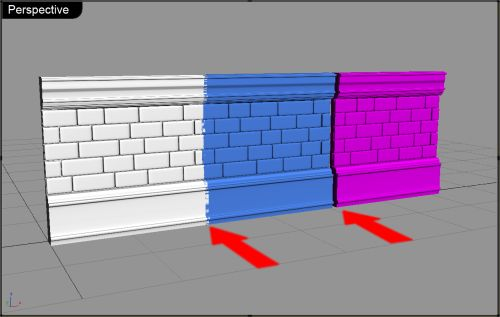
\includegraphics[width=0.9\linewidth]{bilder/glitch}}
  \caption{Beispiel für Überlappung und Lücken zwischen Modulen \parencite{Mader}.}
	\label{glitch}
\end{figure}
\subsection{Nutzerfreundlichkeit}
Damit ein modulares Kit effizient nutzbar ist, muss das Arbeiten mit diesem so angenehm und einfach wie möglich sein. Hierbei ist sehr wichtig, dass sich die einzelnen Teile im Editor einfach bewegen  und verbinden lassen. Nach Möglichkeit sollten diese automatisch einrasten, sobald sie nah genug zusammengeführt werden. \parencite{Mader}.
\par
Auch die Flexibilität trägt erheblich zur Nutzerfreundlichkeit bei. Hierzu zählt, wie kompatibel die einzelnen Teile untereinander sind und wie viel Freiheit sie den Level-Designern lassen. \parencite{unrealModular}.
\par
Zusätzlich lässt sich die Nutzerfreundlichkeit daran messen, wie schnell und einfach größere Strukturen erstellt werden können. \parencite{Mader}.
\subsection{Aufwand}
Kosten spielen bei der Erstellung von Videospielen, wie in jeder Branche, eine große Rolle. Um diese möglichst gering zu halten ist es wünschenswert, den benötigten Arbeitsaufwand und die Zeit zu reduzieren. Effektiv entworfene modulare Assets sind hierfür eine gute Hilfe.
\par
In \textit{Skyrim} wurden über 300 Dungeons\footnote{Ein Dungeon ist ein in sich geschlossenes Level, welches einen Abschnitt der Spielwelt repräsentiert. Das kann z. B. ein verlassener Tempel, eine Höhle oder ein Verlies sein} von nur zehn Personen entwickelt, darunter nur zwei 3D-Artists. Der Einsatz modularer Assets erlaubte dem Team innerhalb der Entwicklungszeit eine große Menge diverser Spielinhalte zu erstellen. \parencite{Burgess}
\par
Ein weiteres Beispiel ist der bereits in Abschnitt \ref{Geschichte von Modularität } erwähnte Einsatz von Modularität in  \textit{For Honor}, bei dem diese genutzt wird, um schnell und einfach Level-Design-Iterationen durchzuführen. \parencite{ForHonor}
\par
Zwar benötigt die Planung modularer Assets vorab mehr Zeit als die Planung herkömmlicher Assets, jedoch ist die Zeitersparnis in der Design-Phase um einiges größer \parencite{Meler}. Ein gutes modulares Asset muss demnach flexibel genug sein, um Level-Design-Iterationen zu beschleunigen.
\subsection{Performance}
Durch das bereits erwähnte \textit{Instancing} (vgl. Abschnitt \ref{Implementierung1}) können modulare Assets helfen, die Performance des Spiels zu verbessern und somit eine höhere Bildfrequenz zu erreichen.
\par
Entscheidend hierfür sind die Modularitätsstufen (vgl. Abschnitt \ref{mstufe}) und die Wiederverwertbarkeit der Assets, damit das Instancing effektiv genutzt werden kann.
\newpage
\subsection{Zusammenfassung}
Die Qualität modularer Assets lässt sich über mehrere Kriterien bewerten. Für den weiteren Verlauf der Arbeit sind die genannten Kriterien ein ausschlaggebendes Bewertungsmaß der erstellten Assets. Hier eine Übersicht der aufgestellten Kriterien:
\begin{itemize}
\item \textbf{Visuelle Qualität}: Lücken und Überlappungen sollten vermieden werden. Um die Kunstermüdung zu vermeiden, sollte das Kit über ausreichend Abwechslung oder musterbrechende Teile verfügen. Starke Wiederholungen sollten vermieden werden.
\item \textbf{Nutzerfreundlichkeit}: Ein gutes modulares Kit ermöglicht einfaches Arbeiten. Zusammenfügen und Bewegen der Teile ist einfach und intuitiv. Die Teile erlauben den Bau größerer Strukturen ohne großen Mehraufwand. Das Kit ist untereinander flexibel und kompatibel.
\item \textbf{Aufwand}: Die Assets helfen in der späteren Projektphase Level Design Iterationen zu verkürzen und ermöglichen die Erstellung einer Vielzahl von Inhalten mit möglichst wenigen Assets.
\item \textbf{Performance}: Das modulare Kit kostet nicht mehr Performance, als ein herkömmliches und erzielt bestenfalls durch Instancing eine noch bessere Performance.
\end{itemize}
\newpage
\section{Methoden für die Generierung modularer Assets}
Um die Planung und die Produktion modularer Kits so effektiv wie möglich zu gestalten, sollten bestimmte Regeln und Vorgehensweisen beachtet werden. Im Folgenden werden die wichtigsten davon erläutert.
\subsection{Projektübergreifende Planung}
Planung ist nach Klafke und Meler einer der wichtigste Aspekt bei der Entwicklung modularer Assets \parencite{Klafke,Meler}.
\par
Sie kann in zwei Stufen eingeteilt werden. Während die erste der beiden Phasen nur einmal im Verlauf des gesamten Projektes durchgeführt werden muss\footnote{\,Dies gilt unter der Annahme, dass alle Kits nach den gleichen Regeln erzeugt werden. Andernfalls muss auch die erste Phase für jedes Kit wiederholt werden.}, muss die zweite für jedes neue Kit im Projekt ausgeführt werden. \parencite{Burgess}
\par
In der ersten Planungsphase werden grundlegende Eigenschaften der angestrebten Modularität festgelegt. Hierzu gehören die verwendeten Modularitätsstufen, die Abstimmung einheitlich verwendeter Rasters \parencite{Perry} und das Setzen der Pivot Points \parencite{Mader}. Auf Grund ihrer Bedeutung und Komplexität werden diese im Folgenden detailliert beleuchtet. Sollten alle erstellten Kits diesen gemeinsamen Regeln folgen, sind sie auch untereinander kombinierbar und können somit für mehr Diversität sorgen \parencite{Burgess}.
\subsection{Modularitätsstufen}\label{mstufe}
Entsprechend des Grades ihrer Aufspaltung in Einzelteile teile L. Perry modular angelegte Assets in verschiedene Stufen (im Original \enquote{Scales}) ein \parencite{Perry}.
\par
Die verwendeten Modularitätsstufen sollten zu Beginn der Planung festgelegt werden, damit die folgenden Schritte einfacher konkretisiert werden können \parencite{unrealModular}.  Die gewählte Stufe ist abhängig von der Spielwelt und dem geplanten Grad der Modularität \parencite{unrealModular}. Wurden diese festgelegt, können die benötigten Gebilde leichter in Module unterteilt werden, die der benötigten Stufe entsprechen. Die Ausprägungen der Stufen werden jetzt erläutert.

\begin{figure}[!h]
\centering
  \makebox[\textwidth]{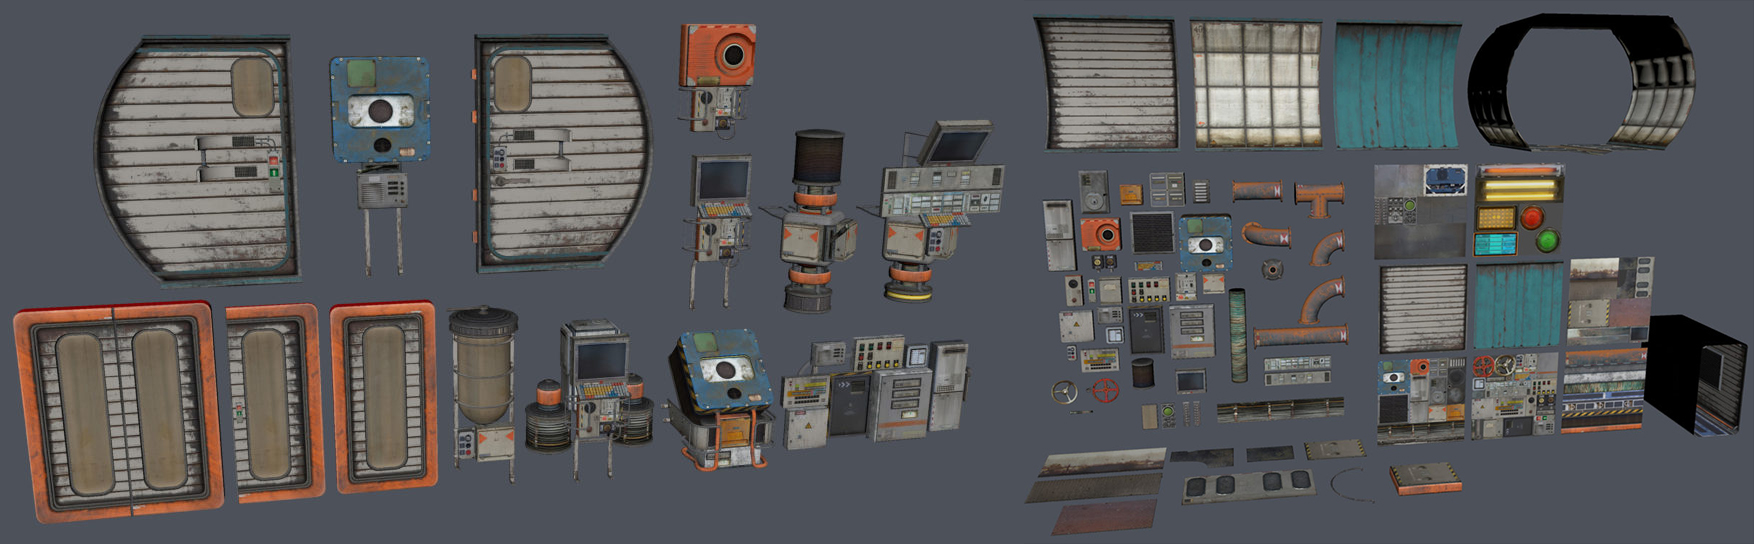
\includegraphics[width=1\linewidth]{bilder/spacemodular}}
  \caption{Module für den Innenraum einer Raumstation. In Anlehnung an \parencite{spacemodular}.}
	\label{spacemodular}
\end{figure}
Für Innenräume empfiehlt sich ein stark granulares Kit, damit Wände, Böden und andere Teile der Umgebung detail- und abwechslungsreich zusammengesetzt werden können. Beispiel für einen solchen Innenraum wäre eine verlassene Raumstation, die nur schleichend erkundet wird \parencite{Perry}.
\par
Abbildung \ref{mittlereStufe} zeigt ein modulares Kit mit mittlerer Modularitätsstufe. Jedes Element aus dem Kit ist eine eigene Wand, mit dessen Hilfe ein Gebäude erstellt werden kann. Eine Mischung aus einer solchen Modularitätsstufe und einer kleineren wurde von  L. Durand für \textit{For Honor} genutzt (vgl. Abbildung \ref{ForHonorImage}).

\begin{figure}[!h]
\label{StufenBilder}
\centering
  \subfloat[][Übersicht eines Kits mit mittlerer Modularität.]{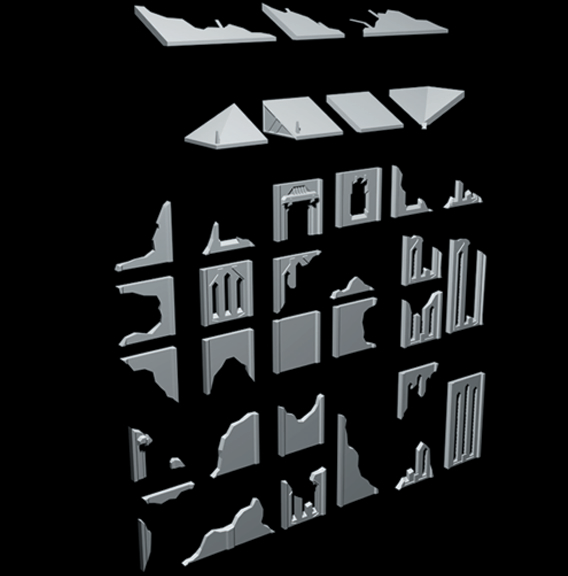
\includegraphics[width=0.45\linewidth]{bilder/ScaleKlein}\label{mittlereStufe}}%
  \qquad
  \subfloat[][Übersicht eines Kits mit geringer Modularität.]{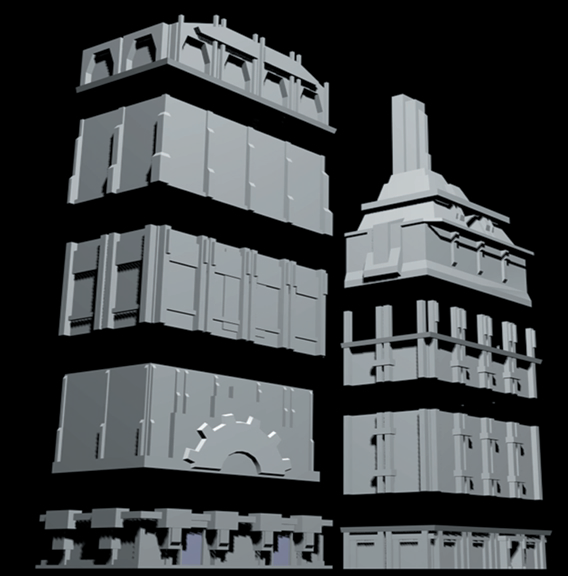
\includegraphics[width=0.45\linewidth]{bilder/ScaleGross}\label{grosseStufe}}%
  \caption{Beispiele für verschiedene Modulraitätsstufen eines Gebäude Kits \parencite{Perry}.}%
\end{figure}
Ein Beispiel für eine geringe Modularitätsstufe zeigt \ref{grosseStufe}. Mit Hilfe dieses Kits können Gebäude aus verschiedenen, vorgefertigten Etagen zusammengesetzt werden. Sie erlauben schnell eine Vielzahl unterschiedlicher Gebäude zu erstellen, jedoch sind diese aufgrund der geringen Modularität recht einseitig.
\par
In der nächstgrößeren Stufe würden ganze Häuser genutzt, um daraus Häuserblöcke zu errichten. Eine weitere Steigerung wäre aus diesen Häuserblöcken eine Stadt zu errichten. Diese Modularitätsstufe eignet sich beispielsweise für den Einsatz in einem Rennspiel. \parencite{Perry}
\par
Innerhalb eines Projekts können durchaus verschiedene Stufen verwendet und gemischt werden. Besitzt ein Spiel beispielsweise offene und geschlossene Bereiche, so ist es sinnvoll, deren Kits unterschiedlich modular zu gestalten. Das gleiche gilt für Bereiche, die der Spieler aus verschiedenen Distanzen sieht. So könnten bei einem Fußweg durch die Stadt beispielsweise die Häuserreihen weniger modular sein als die Straße, über die der Spieler läuft, da letztere deutlich präsenter und näher ist. \parencite{Klafke}
\par
Beim Arbeiten mit nur einer einzigen Stufe kann die Repetition durch die manuelle Platzierung kleinerer Objekte aufgebrochen werden \parencite{Perry}.
\par
Die Modularitätsstufen sollten zudem projektspezifisch betrachtet werden. Für ein Rennspiel im Weltall, dessen kleinste Einheit Raumschiffe sind, ist es wenig sinnvoll die gleichen Modularitätsstufen zu nutzen wie für ein Fantasy-Rollenspiel mit detailliertem Interieur. Die Einteilung der Stufen ist immer auch abhängig von der Spielwelt und Perspektive.
\enlargethispage{10.5pt}
\subsection{Raster}\label{Rasterkapitel}
Nach L. Durand ist einer der wichtigsten Aspekte, für die Umsetzung eines Projekts mit modularem Design, das Raster \parencite{ForHonor}.
\par
Jedes 3D-Tool arbeitet intern mit einem Raster\footnote{\,Das Raster ist hier ein dreidimensionales Koordinatensystem.}. Sie können sich in der verwendeten Maßeinheit (Meter, Zentimeter, Zoll, etc.), der Orientierung des Koordinatensystems, den Unterteilungsstufen und anderen Eigenschaften unterscheiden. Im Raster ist es 3D-Artists möglich, Objekte punktgenau im Raum zu platzieren. Dies ermöglicht die Erstellung modularer Assets mit lückenlosen Übergängen. \parencite{Mader}
\vspace{-10.5pt}
\begin{figure}[H]
\label{RasterBilder}
\centering
  \subfloat[][Beispielhafte Kalkulation der Raster-Einteilungen.]{\includegraphics[width=0.47\linewidth]{bilder/RasterEinteilung}\label{RasterSizes}}%
  \qquad
  \subfloat[][Beispiel für die Angleichung von Modulen.]{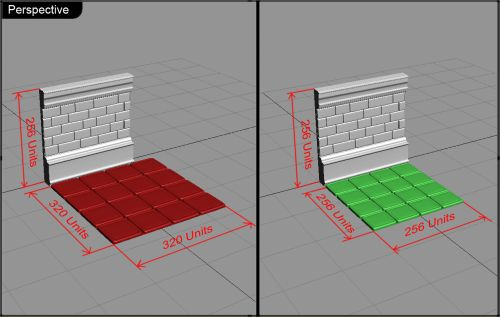
\includegraphics[width=0.47\linewidth]{bilder/GleichGrosseObjekte}\label{sameRasterSize}}%
  \caption{Beispiele für die Anwendung verschiedener Rastergrößen \parencite{Mader}.}%
\end{figure}
\vspace{-10.5pt}
Das Raster sollte möglichst in Stufen von Zweierpotenzen eingeteilt sein. Nur durch das Nutzen von geraden Zahlen kann das Raster in kleinere Stufen aufgeteilt werden. Dies kann für kleinere Objekte nötig sein. Kann die Größe eines Elements nicht durch die standardmäßig genutzte Zweierpotenz dargestellt werden, ist es möglich, kleinere Zweierpotenzen zu addieren oder subtrahieren. Abbildung \ref{RasterSizes} zeigt Beispiele für mögliche Einteilungen des Rasters. \parencite{Mader}
\par
Zu kleine Einteilungen des Rasters, erhöhen jedoch den Aufwand des Zusammenbaus von Elementen. Die Module müssen dann in immer kleineren Schritten über das Raster bewegt werden, wodurch das Einrasten erschwert wird. \parencite{Mader} 
\par
Alle Elemente, die untereinander kompatibel sein sollten, wie beispielsweise Wände, Böden und Decken, sollten die gleichen Grundmaße besitzen, da sie ansonsten nur schwer untereinander kombinierbar sind. \parencite{Mader}
\par
Abbildung \ref{sameRasterSize} illustriert dieses Problem: Die Wand und die rote Bodenfläche sind untereinander nicht kompatibel, ohne dass eines der beiden Elemente größer bzw. kleiner skaliert oder fünf Wand- und vier Bodenelemente benutzt werden. Eine solche Inkompatibilität sorgt für erhöhten Zeitaufwand und eine Einschränkung der kreativen Freiheit der Level-Designer. So verliert sich der Mehrwert der angestrebten Modularität.
\par
Burgess und Purkypile bezeichnen die Grundmaße eines Kits als Footprint (deutsch Fußabdruck). Passt ein Element nicht in den definierten Fußabdruck, sollte es entweder ein Vielfaches oder einen Teiler der Größe des Fußabdruck als Größe nutzen \parencite{Burgess}.
\enlargethispage{10.5pt}
\newpage
Beispielsweise könnte die grüne Bodenfläche aus Abbildung \ref{sameRasterSize} auch die Größe 128x128 besitzen. Dann müssten vier Elemente genutzt werden, um die Fläche vor einer Wand zu füllen, die gewünschte Modularität bliebe zu einem gewissen Grad erhalten.
 \begin{figure}[H]
\centering
  \makebox[\textwidth]{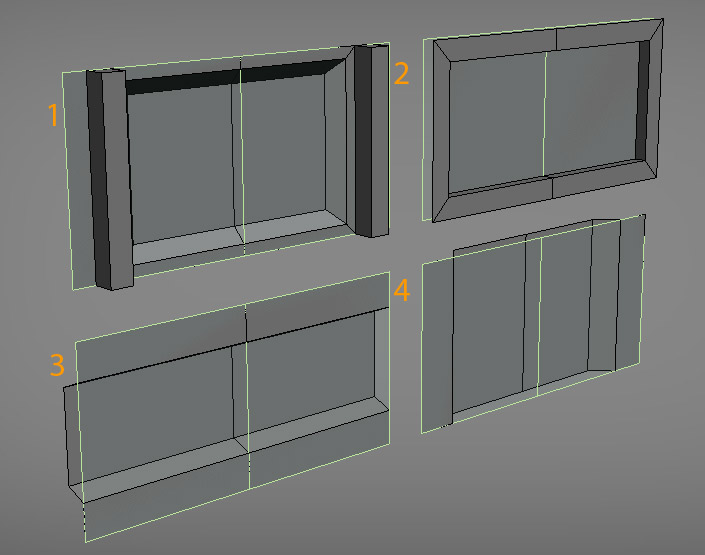
\includegraphics[width=\linewidth]{bilder/boundingBox}}
  \caption{Beispiel für verschiedene Qualitäten von Kontaktpunkte \parencite{Klafke}.}
	\label{boundingBox}
\end{figure}
\vspace{-10.5pt}
Thiago Klafke arbeitet mit \textit{Bounding Boxes}. Alle Module in seinem Kit müssen in eine vorgegebene Box passen. Sie muss nicht in alle Richtungen gefüllt sein, aber ihre Kanten sollten nach Möglichkeit soweit ausgearbeitet sein, dass keine Lücken zwischen den Modulen entstehen. Haben Module eine Tiefe, sollten alle Elemente an den Rändern der \textit{Bounding Box} auf der gleichen Ebene liegen. Abbildung \ref{boundingBox} verdeutlicht dies: Werden z. B. die Elemente 1 und 3 horizontal mit einander verbunden entstehen Lücken. Modul 2 ist in diesem Fall weder mit 1 noch mit 3 oder 4 kombinierbar, da es mit keinem dieser Module verbunden werden kann, ohne Lücken zu erzeugen. \parencite{Klafke}
\par
Die Einteilung der Raster-Größe und seiner Aufteilung sollten abhängig von der Größe der Spielfigur, der Animationen und der Bewegung des Spielers in der Welt entschieden werden \parencite{Perry}. Wenn vorhanden, muss auch die Interaktion von Computer gesteuerten Charakteren mit der Umwelt mit einbezogen werden \parencite{Burgess}. \textit{Skyrim} beispielsweise nutzt als minimale Größe eines begehbaren Elements die Breite von zwei Charakteren, wodurch sichergestellt wird, dass sich alle Figuren frei bewegen können \parencite{Burgess}.
\par
Um die Fehleranfälligkeit zu verringern und den Arbeitsprozess zu beschleunigen, sollten die unterschiedlichen Rasters aller verwendeten 3D-Tools aneinander angeglichen werden. Diese Angleichung sollte optimalerweise direkt im Anschluss an die Konzeption des Rasters erfolgen. \parencite{ForHonor}
\enlargethispage{11.5pt}
\par
\subsection{Positionierung und Nutzen des Pivot Points}
Der Pivot Point (Drehpunkt) oder auch der Origin Point (Ursprung) kann beliebig für jedes Objekt gesetzt werden \parencite[S.\,85]{blender}. Über ihn wird definiert, wo sich das Objekt im Raum befindet und wie sich Rotation, Skalierungen und Spiegelungen darauf auswirken \parencite[S.\,85 \& S.102]{blender}.
\par
Ohne korrekt gesetzten Pivot Point wird die zielgenaue Platzierung eines Objektes im dreidimensionalen Raum erschwert bzw. ist nur eingeschränkt möglich. Ein falsch positionierter Pivot Point schränkt die Vorteile der Modularität ein und beeinflusst den Workflow negativ. \parencite{Mader}
\par
Im Folgenden werden verschiedene Beispiele gezeigt, anhand derer Regeln zur korrekten Platzierung des Pivot Points, für jedes Objekt bzw. Objektgruppe, abgeleitet werden können. Sind Objekte auf einer oder mehreren Achsen symmetrisch, sollte der Pivot Point am Ursprung des lokalen Koordinatensystems des Objekts platziert werden. Dadurch kann mit diesem in der Engine freier gearbeitet werden. \parencite{Mader}
\par
Wie zu fast allem gibt es auch zu der Platzierung des Pivot Points einige fallspezifische Ausnahmen. 
\par
Zusätzlich muss beachtet werden, dass eine nachträgliche Änderung des Pivot Points dazu führt, dass jede Instanz des Objektes im Spiel angepasst werden muss, da z.b. eine Translation des Pivot Points auch zu einer Translation des Objektes in der Spielwelt führt. \parencite{Burgess}
\begin{figure}[H]
\centering
  \makebox[\textwidth]{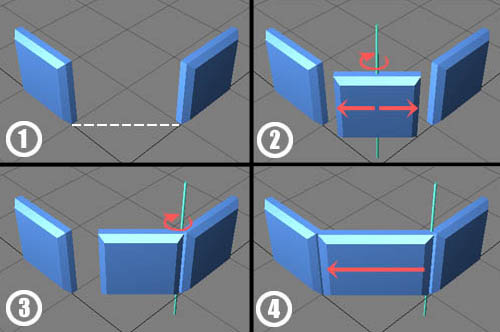
\includegraphics[width=\linewidth]{bilder/cornerPiece}}
  \caption{Beispiel für den Einsatz eines am Ende einer Mauer platzierten Pivot Points \parencite{unrealModular}.}
	\label{cornerPiece}
\end{figure}
\vspace{-10.5pt}
Bei Objekten, die entlang einer Achse wiederholt werden sollen, sollte der Pivot Point möglichst an einem der beiden Enden der Achse positioniert werden (Abbildung \ref{cornerPiece}). \parencite{Mader}
\enlargethispage{10.5pt}
\newpage
Für sich wiederholende Objekte sollte der Pivot Point bei allen Objekten der gleichen Art auf der gleichen Seite der entsprechenden Achse liegen, damit eine einfache Verbindbarkeit der Module gewährleistet ist \parencite{Mader}.
\par
Ein weiteres Beispiel, warum es von Vorteil ist, für Mauer- oder Wandstücke den Pivot Point an einer Seite zu haben, ist das Überbrücken einer Lücke mit einem Winkel. Abbildung \ref{cornerPiece} stellt diesen Fall dar. Wäre der Pivot Point in der Mitte des Moduls, wäre das Anpassen an die Größe der Lücke und das Setzen an die richtige Position mit viel Aufwand verbunden. \parencite{Perry}
\par
Bei, auf dem Boden oder einer anderen Fläche platzierten, Elementen, sollte der Pivot Point möglichst an der Unterseite des Objektes positioniert werden, damit diese bei aktivierter Einrastfunktion auch wirklich mit dem Grund der Spielwelt abschließen. Durch diese Technik können spätere händische Eingriffe verhindert werden. Außerdem ändern diese Objekte dadurch auch nicht ihre Position auf dem Boden, wenn sie skaliert werden. \parencite{Mader}
\begin{figure}[H]
\centering
  \makebox[\textwidth]{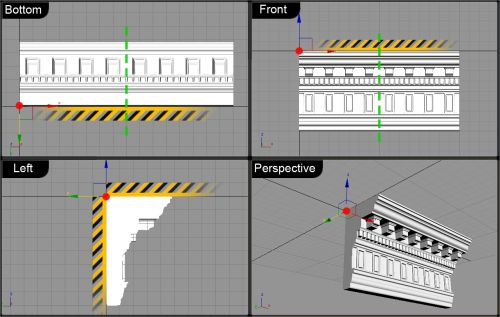
\includegraphics[width=\linewidth]{bilder/stuck}}
  \caption{Beispiel für die Positionierung eines Pivot Points an einer Stuckleiste \parencite{Mader}.}
	\label{stuck}
\end{figure}
\vspace{-10.5pt}
Für Elemente, die unter oder direkt neben anderen platziert werden, sollte der Pivot Point an die Ecke gesetzt werden, die mit den benachbarten Objekten in Kontakt kommen sollen. So kann das Element in genau dieser Ecke einrasten. Ein Beispiel hierfür könnte eine Stuckleiste sein, die zwischen Decke und Wand eingesetzt wird. \parencite{Meler}
\par
Diese Regeln können teilweise auch untereinander kombiniert werden. Soll beispielsweise die Leiste aus dem vorigen Beispiel noch horizontal erweiterbar sein, muss der Pivot Point zusätzlich an einer der äußeren Ecken platziert werden (Abbildung \ref{stuck}). \parencite{Meler}
\newpage
\begin{figure}[H]
\centering
  \makebox[\textwidth]{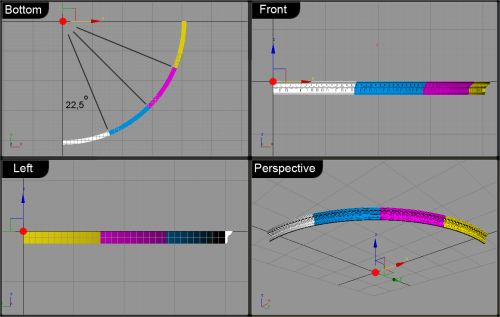
\includegraphics[width=\linewidth]{bilder/pivotRotation}}
  \caption{Beispiel für einen Pivot Point im Zentrum eines Kreises \parencite{Mader}.}
	\label{pivotRotation}
\end{figure}
\vspace{-10.5pt}
Eine etwas unintuitive Ausnahme bilden Objekte mit einer Krümmung in ihrer Oberfläche. Für diese empfiehlt es sich, den Pivot Point in das Zentrum des Kreises der Krümmung zu setzen (Abbildung \ref{pivotRotation}). Dadurch ist er zwar weit weg vom eigentlichen Objekt, allerdings ergibt sich durch die Krümmung ein nützlicher Vorteil: Wenn die Pivot Points der einzelnen Elemente überlagern, können diese durch simple Anpassung der Rotation sehr leicht aneinander angelegt werden. \parencite{Mader}
\subsection{Kit-spezifische Planung}\label{Kit Spezifische Planung}
In der zweiten Planungsphase werden die Details des Kits ausgearbeitet und spezifische Regeln definiert. Während dieser Phase wird das Setting festgelegt, welches das Kit abbilden soll \parencite{Burgess}. Das können beispielsweise vereiste Höhlen oder das Innere eines Raumschiffs sein. Außerdem sollte geklärt werden, wie und mit welchem Zweck das Kit im Spiel eingesetzt wird, damit sein Umfang und seine Möglichkeiten entsprechend planbar sind \parencite{Burgess}. Nach Perry ist es eine gute Methode dafür eine Liste mit allen Eigenschaften, die das Kit erfüllen soll anzufertigen. Dabei geht es primär um die Kernelemente des Kits, welche für den Großteil des Einsatzgebietes genutzt werden \parencite{Perry}.
\par
Einzigartige Modelle, so genannte \textit{Hero Pieces}, sollten erst im späteren Verlauf entwickelt werden. Sie trügen in der frühen Phase wenig zum Fortschritt des Kits bei, benötigten aber viel Arbeit und ihr Fehlen verzögerte im Gegensatz zu den Kernelementen des Kits nur an wenigen Stellen den Arbeitsablauf. \parencite{Burgess}
\par\enlargethispage{30pt}
Joel Burgess fordert in einem GDC-Talk zu validieren, welche Kits eine Existenzberechtigung haben.Können Kits zusammengefasst werden, um ein generalisiertes Kit mit vielseitigerem Nutzen zu erzeugen, sei dies empfohlen. Dies verringere die Anzahl und die Planungszeit der benötigten Kits und so auch die Komplexität des Projekts. \parencite{Fallout4}
\newpage
Perry, Burgess und Purkeypile empfehlen einheitlich, dass Kits Elemente enthalten sollten, mit denen sie untereinander verbunden werden könnten \parencite{Burgess,Perry}. So könne z. B. eine einheitliche Größe für Türrahmen genutzt werden, um den Übergang von einem in das nächste Kit zu schaffen, ohne für beide spezifische Teile anfertigen zu müssen \parencite{Burgess}.
Perry erwähnt zusätzlich, dass Kits abgrenzende Elemente benötigten. So solle für einen modularen Fluss beispielsweise ein Wasserfall oder eine Mündung in ein Gitter existieren, damit der Fluss beendet werden könne \parencite{Perry}. So lange ein Kit nicht für die Generierung endloser Objekte/Level gedacht sei, sei die Einplanung solcher Teile zwingend.
\par
Für das weitere Vorgehen gibt es verschiedene Methoden, bei denen teilweise die Planungsphase in die Erstellungsphase über geht.
\par
Klafke und Norris empfehlen beide, mit der Erstellung von Texturen und Materialien zu beginnen, bevor die ersten Modelle existieren \parencite{Klafke,Norris}. Obwohl sie hier einig sind, unterscheiden sich ihre Vorgehensweisen:
\par
Norris erzeugt für seine Kits bereits voll ausgearbeitete Texturen mit allen Details, die er abbilden möchte, bevor er die Modelle erstellt  \parencite{Norris}. Klafke hingegen arbeitet etwas freier. Für ihn ist ein Mockup der späteren Textur ausreichend, um die Modelle passend zu unwrappen und dadurch im weiteren Verlauf Zeit zu sparen \parencite{Klafke}.
\par
Der Aufbau der genutzten Texturen ist bei beiden ähnlich und besteht aus großen, kachelbaren Texturen, um Wände abzubilden \parencite{Klafke,Norris}. Klafke nutzt diese zusätzlich auch für Bodenflächen \parencite{Klafke}. Für alle im Kit darzustellenden Details erstellen sie eine, beziehungsweise zwei Texturen mit einer Verbindung aus Trims, so genannte Trim Sheets\footnote{\,Trim Sheets sind Texturen, die mehrere unabhängige und meist kachelbare Details enthalten \parencite{Meler}.} \parencite{Klafke,Norris}.
\par
Eine weitere Vorgehensweise wird von Burgess und Purkeypile beschrieben. Hier wird mit der Erstellung einfacher Modelle begonnen, anhand derer alle aufgestellten Regeln und erarbeiteten Ideen ausgiebig getestet werden. Es ist möglich, dass in dieser Phase viele Modelle entstehen, die verworfen werden, bevor eine Herangehensweise gefunden wird, um passende Assets zu erstellen. In dieser Zeit können die Regeln des Kits noch einfach verändert  und auf die Bedürfnisse des Spiels angepasst werden. \parencite{Burgess}
\par
Die nächste Stufe dieses Prozesses ist das sogenannte \textit{Grayboxing}. In dieser Phase werden die Kernelemente des Kits mit einem geringen Detailgrad und ohne Texturen erstellt. Das \textit{Grayboxing} dient weiterhin dazu, das Konzept des Kits sowie die Funktionen der einzelnen Module zu überprüfen und solange zu verfeinern, bis alle Elemente auf dem gewünschten Niveau sind. Die visuelle Qualität der Elemente spielt dabei noch keine große Rolle, der Fokus liegt auf der Funktionalität. Können die Elemente des Kits alle Probleme lösen, für die es konzipiert wurde, kann die Phase beendet werden. \parencite{Burgess}
\par
Nach der \textit{Graybox}-Phase werden alle Assets ausgearbeitet. Aus den vorher entworfenen Elementen werden detailreiche, texturierte Assets erstellt und für die weitere Verarbeitung freigegeben. Zusätzlich werden weniger prominente Teile erstellt, die in der vorherigen Phase ausgelassen wurden. Existieren Varianten von Assets, sollte erst eine Version fertig gestellt werden, um final testen zu können, dass es keine Probleme gibt. So kann vermieden werden, dass alle Varianten überarbeitet werden müssen, wenn es zu Fehlern kommt. Sowohl während dieses Vorgangs als auch danach werden alle Assets verfeinert. Es werden bestehende Fehler und Unreinheiten ausgebessert und die Kits, falls nötig, um Module erweitert, bis das Projekt beendet ist. \parencite{Burgess}
\par
Eine dritte Vorgehensweise wird von Perry angeführt. Ihm zufolge sollten erst einfache modulare Modelle erstellt und dann nach und nach weitere komplexere Teile hinzugefügt werden. Unterstützend zu dieser Arbeit soll eine Asset-Review eingeführt werden, bei der regelmäßig getestet wird, ob alle bisher produzierten Modelle wie vorgesehen untereinander kompatibel sind und funktionieren. Dies soll gewährleisten, dass am Ende keine fertigen Assets erzeugt werden, die nicht ohne aufwändige Überarbeitungen funktionieren. \parencite{Perry}
\par
Ein bisher unerwähnter Aspekt ist die Namensgebung der modularen Assets. Bereits früh im Projekt sollte eine passende Namenskonvention eingeführt werden, die auf alle Kits anwendbar ist. Dies sorgt dafür, dass alle Artists, Designer und Programmierer immer genau wissen, welchen Zweck ein bestimmtes Modul hat und damit schneller und effizienter arbeiten können. \parencite{Burgess}

\begin{figure}[!h]
\centering
  \makebox[\textwidth]{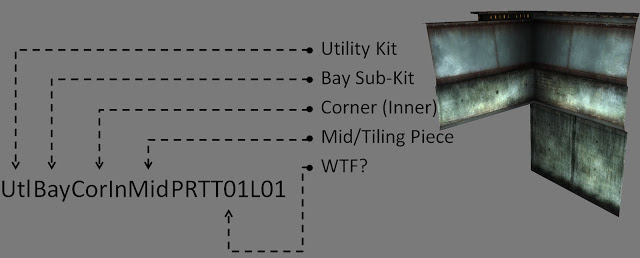
\includegraphics[width=\textwidth]{bilder/namingConvention}}
  \caption{Beispiel für Namensgebung eines modularen Assets aus \textit{Fallout 3} \parencite{Burgess}.}
	\label{namingConvention}
\end{figure}
Abbildung \ref{namingConvention} zeigt beispielhaft die Kodierung einer Namenskonvention. Der Name sollte möglichst deskriptiv und einfach zu entschlüsseln sein. Zudem ist es sinnvoll, eine bei \enquote{01} beginnende und aufsteigende Nummerierung einzuführen. Dies erleichtert die spätere Implementierung von Asset-Varianten. Durch die Einhaltung der Namenskonvention teilen sich alle Elemente einer Art einen Namen. Dies reduziert die Komplexität des Systems und Elemente können durch einfaches Heraufzählen ausgetauscht werden. \parencite{Burgess}
\par
Alle wichtigen Aspekte der Planung und Grundlagen für Modularität sind jetzt erklärt. In den folgenden Abschnitten werden weitere, für die Generierung modularer Assets hilfreiche Aspekte erläutert. 
\subsection{Weitere Techniken}\label{weitereT}
In diesem Abschnitt werden weitere Methoden erläutert, die keinem der obigen Themen zuzuordnen oder nur in Randfällen anwendbar sind.
\par
Bei der Nutzung modularer Assets sollte man  auch außerhalb der vorgegebenen Regeln denken und Module von Zeit zu Zeit zweckentfremden. So könne beispielsweise eine Zimmerpflanze auch als Baum eingesetzt werden, wenn die Distanz zum Spieler ausreichend sei. \parencite{unrealModular}
\par
Module können direkt so gestaltet werden, dass sie mehrere aufgaben erfüllen können. Zum Beispiel könnte die Decke einer Höhle gleichzeitig auch als Boden genutzt werden \parencite{Perry}. Dadurch könnten mit etwas mehr Planung Ressourcen und Arbeitszeit eingespart werden \parencite{unrealModular}.
\par
Um das rasterartige Erscheinungsbild modularer Assets zu mildern, kann an manchen Stellen das Raster verlassen werden. Dies ist allerdings nur möglich, wenn der Editor es auch technisch erlaubt. Für das Platzieren von Modulen im Editor kann definiert werden, dass Objekte an einem alternativen Raster, welches durch die Rotation und Position eines gewählten Elementes definiert wird, ausgerichtet werden. \parencite{Burgess}
\par
Kits sollten außerdem Elemente enthalten, die eventuelle Lücken oder unschöne Übergänge\footnote{\,Diese können zum Beispiel durch Texturen entstehen, die nicht zueinander passen oder durch Module die nicht füreinander konzipiert wurden.} verbergen. Diese helfen auch repetitive Muster des Kits zu brechen. Beispiele dafür sind Säulen, Pfeiler, Steinformationen oder auch Pflanzen. \parencite{Burgess,Perry}
\par
Falls geplant ist das normale Raster zu verlassen, müssen zusätzlich Elemente entworfen werden, die Lücken und Kanten verbergen. Werden beispielsweise in verschiedenen Winkeln verbundene Tunnel-Elemente genutzt, müssen Übergänge für alle Möglichkeiten erstellt werden, wie diese verbunden werden können. \parencite{Burgess}
\vspace{-10.5pt}
\begin{figure}[H]
\centering
  \subfloat[][Textur ohne den Einfluss von Vertex Farben.]{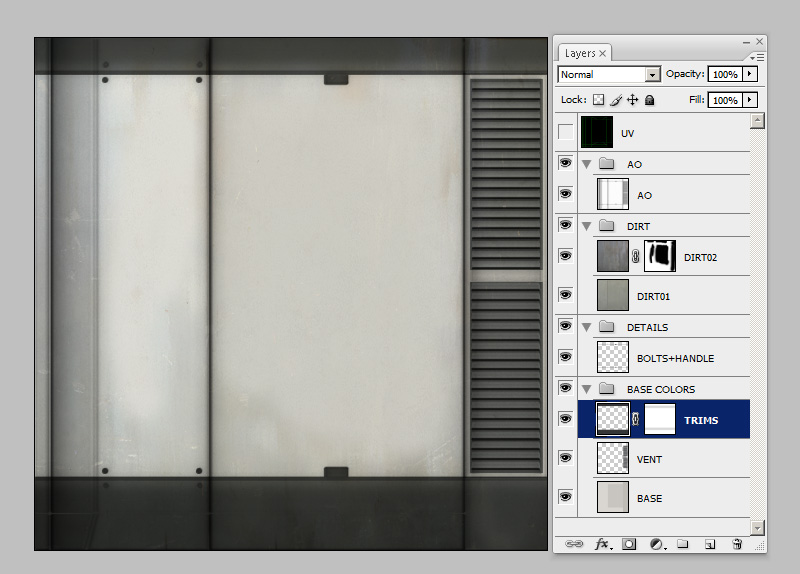
\includegraphics[width=0.415\linewidth]{bilder/vertexColorNoColor}\label{vertexColorNoColor}}%
  \qquad
  \subfloat[][Assets unter dem Einfluss Vertex Farben.]{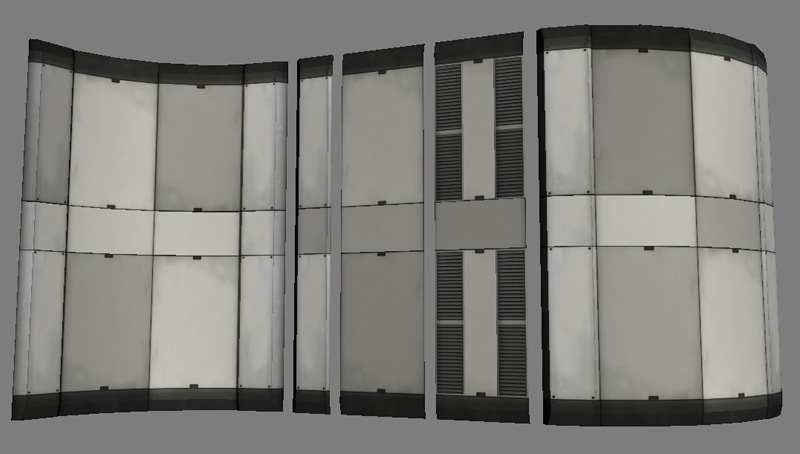
\includegraphics[width=0.525\linewidth]{bilder/vertexColor}\label{vertexColor}}%
  \caption{Beispiele für Einfluss von Vertex Farben \parencite{Klevestav}.}%
\end{figure}
\vspace{-10.5pt}
In 3D-Tools kann Vertices eines Meshes ein Farbwert zugeordnet werden. Diese Farbwerte heißen Vertex-Farben. Durch diese Technik kann, ohne großen Aufwand und ohne neue Objekte eine größere Anzahl Modelle erzeugt werden. In den Material-Einstellungen des Objekts muss angegeben werden, dass für die Farbgebung des Models die Vertex-Farben einkalkuliert werden sollen. Die Abbildungen \ref{vertexColorNoColor} \and \ref{vertexColor} zeigen, wie sich diese auf das Aussehen einer Textur auswirken können. \parencite{Klafke,Klevestav}
\subsection{Texturierung  von modularen Assets}
In dieser Thesis liegt der Fokus auf der Arbeit an den Modellen. Texturierung wird demzufolge nur angeschnitten.
\par
\begin{figure}[H]
\centering
  \makebox[\textwidth]{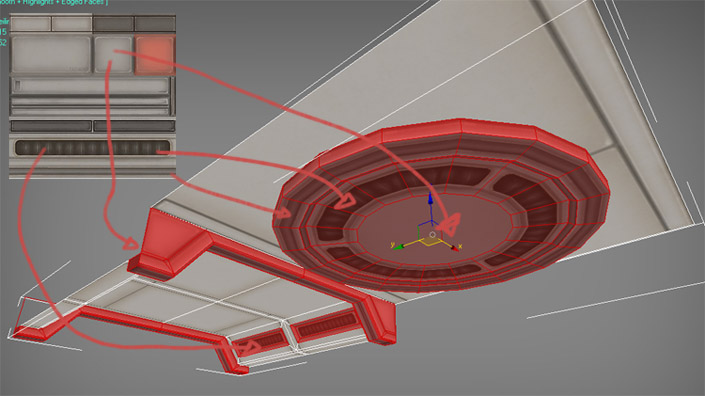
\includegraphics[width=0.72\linewidth]{bilder/trims}}
  \caption{Beispiel für Mehrfachnutzung eines Trimsheets \parencite{Klafke}.}
	\label{trims}
\end{figure}
\vspace{-10.5pt}
Modulare Elemente können wie normale Assets texturiert werden. Texturen von gemeinsam genutzten Objekten sollten aus Performance-Gründen auf einem Textur-Atlas verbunden werden. Nutzt ein Projekt Elemente, die mehrfach aneinandergefügt werden sollen, bietet es sich an, kachelbare Texturen zu nutzen. Auf diese Weise können große Flächen erzeugt werden, ohne Kanten oder sichtbare Nähte. Dies ist vor allem für modulare Assets von großem Vorteil. Da sie vielseitig nutzbar sind und nur einmal geladen werden müssen, sparen solche Texturen außerdem Ressourcen. \parencite{Meler}
\par
\begin{figure}[H]
\centering
  \makebox[\textwidth]{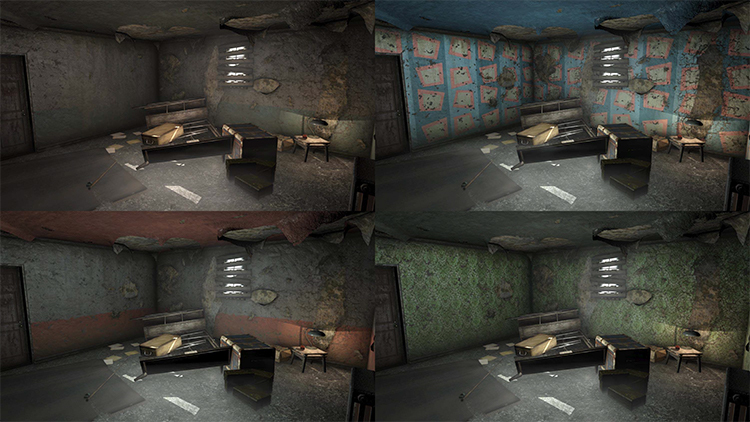
\includegraphics[width=0.72\linewidth]{bilder/MaterialSwap}}
  \caption{Ein Beispiel für das Potential austauschbarer Texturen. In Anlehnung an \parencite{Fallout4P}.}
	\label{MaterialSwap}
\end{figure}
\vspace{-10.5pt}
Werden austauschbare Texturen genutzt, die dem gleichen Aufbau folgen, kann ein Modell unterschiedlich aussehen. \parencite{Norris}
\par
Hiermit sind die Grundlagen für die praktische Ausarbeitung dieser Thesis abgeschlossen. Die nachfolgenden Kapitel wenden diese in der eigenen Umsetzung modularer Assets an.
\enlargethispage{11.5pt}
\chapter{Beispielanwendung}
\section{Das Spiel}
Dieser Abschnitt soll einen grundlegenden Überblick über das Spiel gewähren, für welches die modularen Gebäude erstellt werden. Die folgenden Abschnitte behandeln die Anwendung der zuvor erarbeiteten Methoden.
\begin{description}
\item[Grundlagen]~\par
Bei \textit{Renegade Line} handelt es sich um einen Third Person Cartoon Shooter, in dem bis zu 16 Spieler über das Internet in verschiedenen Spielmodi auf unterschiedlichen Karten gegeneinander spielen können. In den meisten Spielmodi werden die Spieler in zwei Teams mit jeweils acht Spielern eingeteilt, die im Anschluss um den Sieg kämpfen. Spieler können während des Spiels eine von vier verschiedenen Klassen wählen, die spezielle Fähigkeiten und passende Waffen besitzen.
\par
Das Spiel befindet sich zum Zeitpunkt dieser Thesis im Early Access und wird von Raw Vengeance Studios entwickelt. Raw Vengeance ist ein kleines Start-up aus Hamburg. Aktuell wird eine neue Karte für einen neuen Spielmodus entwickelt. Zusammen mit der neuen Karte soll auch ein neues Setting etabliert werden. Bisher wurden alle Modelle für die neue Karte von mir erstellt.
\item[Der Stil]~\par
Der Stil des Spieles ist ein stilisierter Cartoon Look. Alle Elemente sind Abwandlungen ihrer realen Gegenstücke. Meist werden prägnante Formen stark hervorgehoben. Das bisherige Setting aller Assets ist leicht stereotypisierend an eine italienische Kleinstadt angelehnt (vgl. Abbildung \ref{altSetting}). Das neue Setting soll das feudale Japan repräsentieren. Auch hier wird mit Stereotypen gearbeitet, die eindeutig und leicht zu erkennen sein sollen. In \textit{Renegade Line} können Gebäude nicht betreten werden, alle Handlungen finden im Freien stattfinden. Dies reduziert die Komplexität der Modelle und die Arbeitszeit ihrer Erstellung.
\end{description}
\enlargethispage{12pt}
\begin{figure}[H]
\centering
  \makebox[\textwidth]{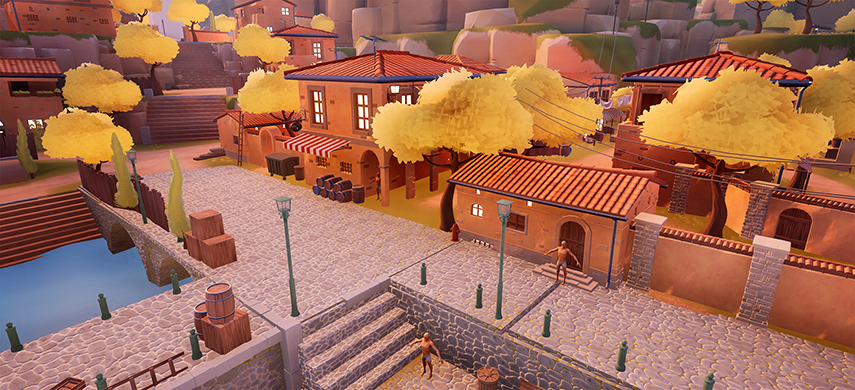
\includegraphics[width=\linewidth]{bilder/altSetting}}
  \caption{Ausschnitt eines aktuellen Levels in dem bisherigen Setting.}
	\label{altSetting}
\end{figure}
\vspace{-10.5pt}
\newpage
\section{Planung}
In der Planungsphase wurde in Zusammenarbeit mit dem Lead-Level-Designer definiert, welche Anforderungen das Kit erfüllen soll. Es wurde über den generellen Aufbau der Gebäude gesprochen. Dies umfasst die Größe der Grundrisse, die Anzahl der Stockwerke, welche Elemente eine Etage ausmachen sollen und welche Sonder-Elemente es geben soll. Außerdem wurde das Design der verschiedenen Elemente angesprochen. Die Umsetzung der Anforderungen habe ich selbst ausgearbeitet.
\par
Diese Anforderungen wurden festgelegt:
\begin{description}
\item[Grundriss]\hfill
\begin{itemize}[leftmargin=0cm]
\item Gebäude sollen nicht nur rechteckig, sondern auch in anderen Formen aufgebaut sein (L-Form, Kreuz etc..) und
\item die Grundfläche eines Gebäudes soll nach Möglichkeit unlimitiert sein.
\end{itemize}
\item[Etagen]\hfill
\begin{itemize}[leftmargin=-0cm]
\item Es sollen mindestens fünf oder besser unbegrenzt viele Etagen möglich sein und
\item in der untersten Etage soll ein Steinfundament mit einer Treppe eingesetzt werden können.
\end{itemize}
\item[Details]\hfill
\begin{itemize}[leftmargin=-0cm]
\item Es soll Elemente für ein Vordach geben, das eine Art Umrandung um das Gebäude bildet (Abbildung \ref{KitelementeSkizze} auf Seite \pageref{KitelementeSkizze} ),
\item Wandstücke sollen in verschiedenen Ausführungen erstellt werden: mit unterschiedlichen Holzmustern, Fenstern und Türen und
\item es soll Elemente für einen Balkon geben, wenn möglich.
\end{itemize}
\item[Design]\hfill
\begin{itemize}[leftmargin=-0cm]
\item Die Farbgebung soll sich an Abbildung \ref{JapanKonzept} (Folgeseite) und dem bisherigen Farbspektrum orientieren und
\item das grundlegende Design der Gebäude soll sich an Abbbildung \ref{JapanKonzept} (Folgeseite) und Abbildung \ref{KitelementeSkizze} (Seite \pageref{KitelementeSkizze}) orientieren.
\end{itemize}
\end{description}
\begin{figure}[!h]
\centering
  \makebox[\textwidth]{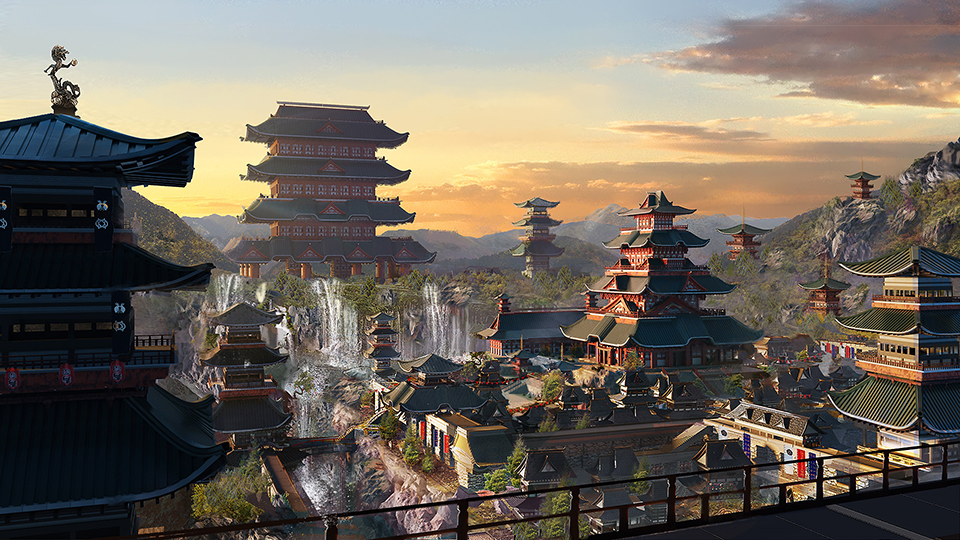
\includegraphics[width=\linewidth]{bilder/Konzept}}
  \caption{Konzept für Farbgebung und Aufbau der Gebäude \parencite{JapanConcept}.}
	\label{JapanKonzept}
\end{figure}
\newpage
Nach der konzeptionellen Planung wurde geprüft, welche Möglichkeiten die genutzten Programme bieten, um das Projekt umzusetzen. Zudem wurden erste Einstellungen vorgenommen, um einen fehlerfreien Ablauf nachfolgender Prozesse zu gewährleisten. Die Maßeinheiten von Blender und UE wurden aufeinander abgestimmt und die \textit{Snapping}-Funktion in UE getestet.\footnote{\,Für dieses Projekt wurde mit Blender 2.79b und Unreal Engine 4.21.2 gearbeitet}
\par
In UE wurde bisher mit Zentimetern gearbeitet, dies wird so beibehalten. Für das Arbeiten mit einem modularen System wird das Raster von klassisch (mit Schritten von 1 m, 2 m, 5 m usw.) auf die Basis von Zwei und dessen Potenzen eingestellt. Abstände, die so entstehen, lassen sich, wie in Abschnitt \ref{Rasterkapitel} erwähnt, besser halbieren ohne das ungerade Zahlen entstehen, die das genaue Platzieren von Objekten deutlich erschweren würden. Durch eine einfache Einstellung im Viewport\footnote{\,Der Viewport ist eine grafische Oberfläche, in dem das aktuelle Level betrachtet und bearbeitet werden kann} kann die Raster Größe (2 cm, 4 cm, 8 cm, ... 128 cm, 256 cm, usw.) angepasst werden.
\par
Auch in Blender kann die Maßeinheit auf Zentimeter eingestellt und das selbe Raster wie in UE konfiguriert werden. Das Raster wird hier allerdings nur wenig benutzt: Beim Modellieren ist es eher hinderlich, wenn Bewegungen nur in definierten Schritten durchgeführt werden können, da viele Details der Modelle dem Raster nicht folgen werden.
\par
Die Planung der Elemente basiert auf den Eigenschaften bestehender Assets. Durch dieses Vorgehen soll sichergestellt werden, dass sich die neuen Modelle in den bestehenden Stil einfügen.
\par
Die bisherigen Gebäude wurden für ein anderes Setting entwickelt, die genutzten Maße gelten dennoch als Orientierung für die neuen Assets.
\newpage
\begin{description}
\item[Größen bestehender Elemente]\hfill
\begin{itemize}[leftmargin=0cm]
\item Türen sind 2,8 m hoch und 1,8 m breit,
\item Fenster sind zwischen 1,5 m und 2,4 m hoch und breit,
\item eine Etage der alten Gebäude ist ca. 4,3 m hoch,
\item Treppenstufen an Gebäuden haben eine Höhe  von ca. 24 cm und eine Tiefe von ca. 27 cm,
\item Treppenstufen in der Welt haben eine Höhe  von ca. 42 cm und eine Tiefe von ca. 56 cm und
\item die Spielfiguren sind 195 cm hoch und ca. 70 cm breit.
\end{itemize}
\end{description}
Als Fußabdruck (siehe Abschnitt \ref{Rasterkapitel}) für die neuen Elemente wird eine Größe von 5,12 m x 5,12 m x 5,12 m genutzt. Kein erstelltes Element soll den so definierten Würfel überschreiten.
\par
Auf Grundlage der bestehenden Gebäude wurde sich für eine Etagenhöhe von 5,12 m entschieden. Grund hierfür war die ursprüngliche Etagenhöhe von 4,3 m, zu der für die neuen Gebäude noch die Höhe des Vordaches addiert wird. Nach längerer Planung habe ich mich für Elemente entschieden, die so aufgebaut sein sollen, wie in Abbildung \ref{KitelementeSkizze} eingezeichnet. In der Modelierungsphase wurde erkannt, dass dieser Ansatz eher ungeeignet ist um das volle Potenzial von Modularität auszunutzen. Im nächsten Abschnitt wird auf den alternativen Lösungsansatz eingegangen.
\par\enlargethispage{14pt}
Damit das Kit mehr Abwechslung erzeugen kann, wurden zudem Elemente in halber Höhe (2,56 m) und halber Breite (2,56 m) geplant. Ein schon in der Planungsphase erkennbares Problem, war das Zusammenlaufen der Etagen. Der Prozess zur Lösung dieses Problems wurde in die Modellierungsphase verschoben. Es erschien leichter, eine Lösung im dreidimensionalen Raum zu finden, statt mit Skizzen zu arbeiten.
\enlargethispage{14pt}
\vspace{-4pt}
\begin{figure}[H]
\centering
  \makebox[\textwidth]{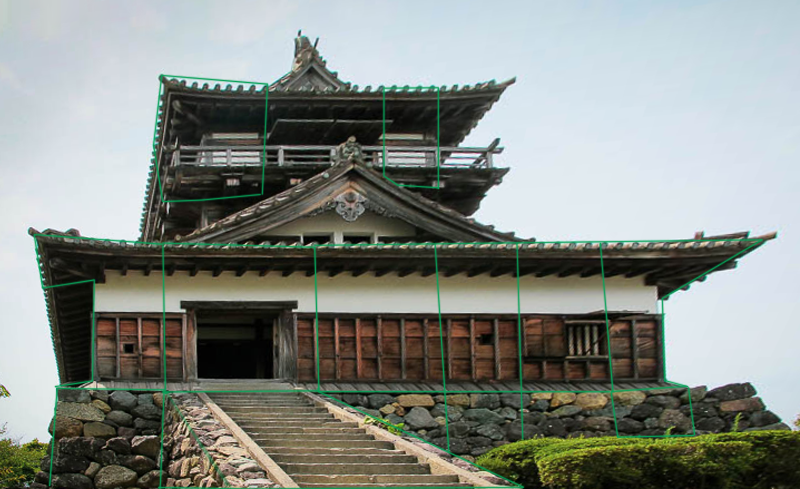
\includegraphics[width=\linewidth]{bilder/KitelementeSkizze}}
  \caption{Skizze der zunächst definierten Module. In Anlehnung an \parencite{KitelementeSkizze}.}
	\label{KitelementeSkizze}
\end{figure}
\vspace{-12pt}
\newpage
Für das Projekt wurde eine mittlere Stufe von Modularität gewählt. Weitere Varianz wird durch verschiedene Versionen der gleichen Elemente erzeugt. Zusätzlich werden kleinere Module erstellt, um Muster aufzubrechen und den Gebäuden mehr Details zu verleihen. Bisher wurden neun verschiedene Gebäude für alle Level genutzt, aufgrund der Perspektive und der Art des Gameplays ist dies bisher nur gering negativ aufgefallen. Folglich sollte es unproblematisch sein, wenn die neuen Gebäude, aus der genutzten Spielperspektive, aus größeren Elementen bestehen, auch wenn es weniger Abwechslung bedeutet.
\par
Das Kit wurde für eine bessere Übersicht und leichtere Handhabung in sieben Subkits aufgeteilt. Die Sets entsprechen jeweils einer Ebene des Gebäudes.
\begin{table}[H]
\fontsize{9}{11}\selectfont
\centering
\begin{tabular}{| l | l |}
\hline\par
\textbf{Subkit}&\multicolumn{1}{c |}{\textbf{Bedeutung}}\\ \hline
Fundament&Elemente für das optionale Steinfundament \\ \hline
Wall&Wandelemente\\ \hline
Balcony&Balkonelemente\\ \hline
Roof&Elemente für das optionale Dach\\ \hline
TopRoof&Dachelemente\\ \hline
Joist&Dachbalkenelemente, die auf das Dach gesetzt werden können\\ \hline
Beam&Holzbalkenelemente, die an Wandübergängen platziert werden können\\ \hline
\end{tabular}
\caption{Übersicht aller Subkits und deren Bedeutung}
\end{table}
\vspace{-10.5pt}
Die Benennung der Elemente, ist wie in Abschnitt \ref{Kit Spezifische Planung} erwähnt, ein wichtiger Faktor für effizientes Arbeiten mit modularen Kits. Für die Bezeichnung wurden verschiedene Begriffskategorien definiert, mit deren Hilfe die Elemente genau zugeordnet werden können. Der Name eines Moduls setzt sich aus den folgenden Kategorien zusammen:
\begin{table}[H]
\fontsize{9}{11}\selectfont
\centering
\begin{tabular}{ l  l  l  l  l }
Subkit & Höhe & Form & Breite & Variante\\ \hline
Ro(of) & Ha(lf) & In(ner Corner) & Si(ngle) & 04
\end{tabular}
 \caption{Bezeichnungsschemata der genutzten Module mit einem Beispiel}
\end{table}
\vspace{-10.5pt}
Zuerst wurde versucht die Bezeichnungen der Elemente nur aus den Anfangsbuchstaben der Wörter zu bilden, die ein Modul ausmachen (z. B. \enquote{FSBS01}). Es stellte sich heraus, dass eine so starke Vereinfachung schwer zu lesen beziehungsweise zu erlernen ist. Aus diesem Grund wurden für die Benennung der Elemente die ersten beiden Buchstaben genutzt, um die Namen der Elemente zu generieren. Aus \enquote{FSBS01} wurde \enquote{FuSiBaSi01}, welches einfacher in \enquote{Fundament Single Basic Single 01} übersetzt werden kann.
\par
Die Bezeichnung der Höhe wurde so weit vorne im Namen platziert, damit bei einer Suche im Editor zusammengehörige Elemente leicht gefunden werden können. Die verschieden hohen Elemente können auf einer Ebene nicht miteinander verbunden werden. Durch dieses Schema können die nicht kompatiblen Elemente leicht voneinander getrennt werden.
\par
Der Abschnitt zur Planung ist hier beendet, die Planung insgesamt jedoch noch nicht und wird während der Modellierung fortgeführt. Die geplanten Konzepte müssen mit einfachen Modellen getestet und eventuell angepasst werden. Nur so können im späteren Verlauf Fehler vermieden werden.
\enlargethispage{10.5pt}
\section{Modellierung}
Zu Beginn der Modelierungsphase wurden Prototypen der konzipierten Modelle erstellt und auf ihre Funktion hin überprüft.
\par
Das zuvor entwickelte System funktionierte. Durch das Einhalten der definierten Größen und das Platzieren der Pivot Points an den unteren Eckpunkten der Module ließen sich die Objekte leicht miteinander verbinden ohne das Lücken entstanden.
\par
Um zu überprüfen, ob das Kit auch in der UE funktioniert, wurden die Module testweise importiert und zu einem Gebäude verbunden (Abbildung \ref{ErsterTestInUnreal}). Auch in der Engine traten keine Probleme mit dem Kit auf. Das Raster in UE wurde auf 1.28 m eingestellt, was das Zusammensetzen des Gebäudes enorm beschleunigte.
\begin{figure}[H]
\centering
  \subfloat[][Alle Prototypen-Module in Blender.]{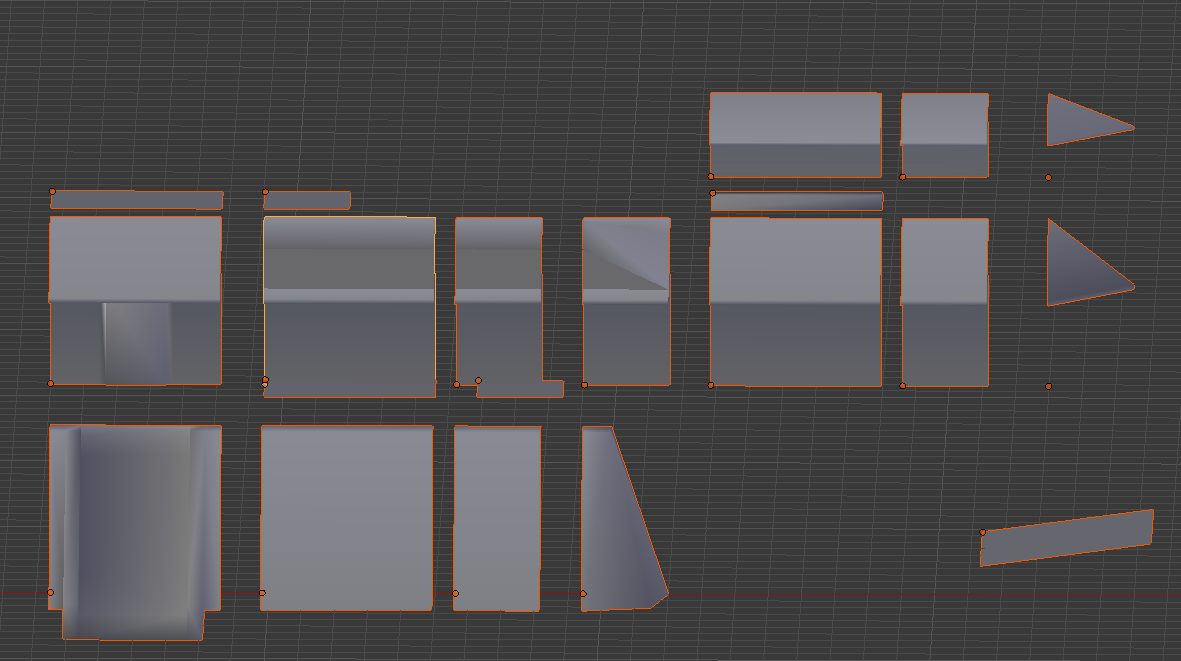
\includegraphics[height=4.22cm]{bilder/ErsterModulTest}\label{ErsterModulTest}}%
  \qquad
  \subfloat[][Aus Modulen erstelltes Gebäude in UE.]{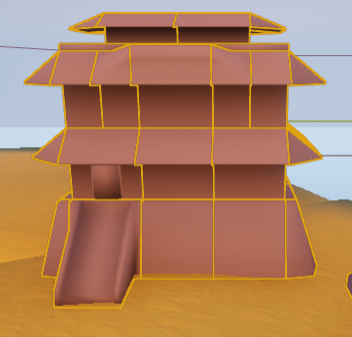
\includegraphics[height=4.22cm]{bilder/ErsterTestInUnreal}\label{ErsterTestInUnreal}}%
  \caption{Erste Prototypen der geplanten Module.}%
\label{ErsterModulTest}
\end{figure}
\vspace{-10.5pt}
\begin{wrapfigure}{l}{0.5\textwidth}
  \centering 
  \vspace{-11.5pt}
    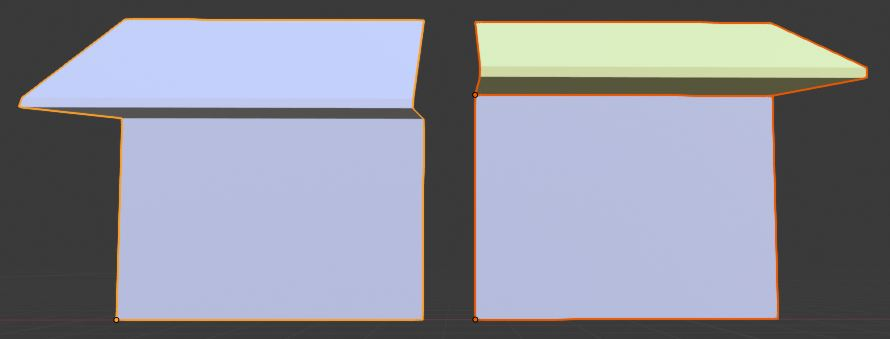
\includegraphics[width=0.5\textwidth]{bilder/Wallrework}
      \caption{Ursprüngliches Wandelement (links) und überarbeitete Version mit abgelöstem Dach (rechts).}\label{Wallrework}
          \vspace{-10pt}
\end{wrapfigure}
Im Anschluss wurde begonnen, die Module weiter auszubauen. Dabei wurde klar, dass die geplante Struktur der Module die Modularität des Kits einschränken und den Arbeitsaufwand vergrößern würde. Es war geplant, dass jedes Wandmodul mit einem Dach oder einem Dach und einem Balkon erstellt werden sollte. Ein besserer Ansatz ist es, die Dächer und Balkone von den Wänden zu trennen, was zur Folge hat, dass die Wände nicht mehr eine Höhe von 5,12 Metern haben. Um das Raster nicht zu verlassen, wurde die normale Größe von Wänden auf 3,84 Metern gesetzt. Zusammen mit Dachelementen, die 1,28 Meter hoch werden, kann die Etagenhöhe von 5,12 Metern wieder eingehalten werden. Die zuvor geplanten halbhohen Wandelemente werden mit einer Höhe von 2,56 Metern erstellt. 
\newpage
\begin{wrapfigure}{l}{0.35\textwidth}
\centering 
  \vspace{-0.5pt}
    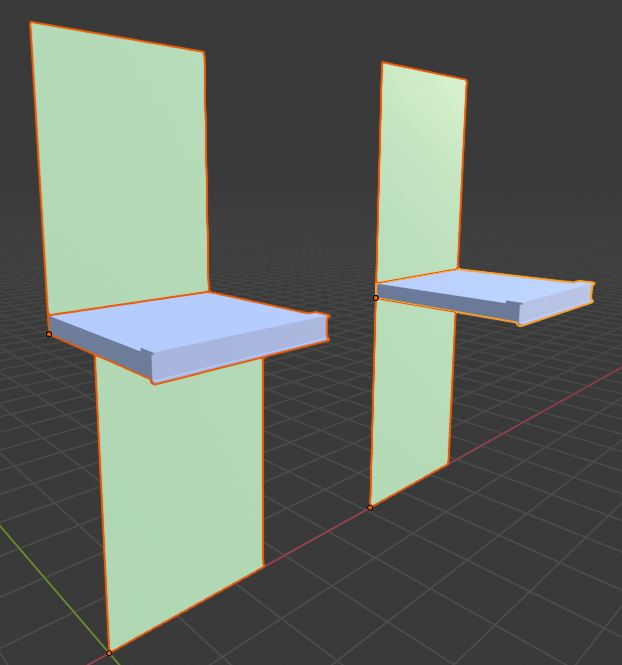
\includegraphics[width=0.35\textwidth]{bilder/balconposition}
      \caption{Mögliche Kombinationen von Balkon- und Wandelementen.}\label{balconposition}
      \vspace{-14pt}
\end{wrapfigure}
Durch diese Änderung konnte die Anzahl der benötigten Module verringert und die Modularität des Kits erhöht werden. Bei Bedarf können Wandelemente auch ohne Dachelemente aufeinander gesetzt werden, um größere Wände zu erzeugen. Auch Balkonmodule können durch diese Entwicklung vielseitiger genutzt werden. Sie können entweder an die Wand gesetzt werden oder auch 1,28 Meter nach innen in das Gebäude verschoben werden, um die nachfolgende Etage zu verkleinern, ohne dass hierfür verschiedene Module benötigt werden.
\par
\begin{wrapfigure}{l}{0.35\textwidth}
\centering 
  \vspace{-11.5pt}
    \includegraphics[width=0.35\textwidth]{bilder/holzecke}
      \caption{In Wandelemente eingesetzte Holzbalken mit Sonderelement.}\label{holzecke}
      \vspace{-14pt}
\end{wrapfigure}
Nach der Überarbeitung des Systems wurden die neuen Wandelemente mit einem halben vertikalen Holzbalken am linken und rechten Rand erweitert. Werden zwei Elemente miteinander verbunden, bildet sich am Übergang ein vollständiger Holzbalken. Die Holzbalken wurden eingesetzt, um das Kit dem Setting anzupassen. Wurde mit Wandmodulen eine Ecke gebildet, entstand eine Lücke zwischen den Holzbalken, die mit einem Sonderelement gefüllt werden musste.
\par
Bei einem weiteren Test in UE wurden Probleme mit Schatten gefunden. An Stellen, bei denen Module aufeinander treffen und keinen glatten Übergang bilden, kommt es zu sehr starken Helligkeitsunterschieden, die falsch aussehen. Dies passierte bei dem Element zum Füllen der Lücke zwischen Holzbalken und bei der bis dahin genutzten Form von Eckelementen der Dachmodule. Dieses Problem kann auch bei glatten Übergängen auftreten, ist dort aber weniger auffällig.
\par
Die Form der Dachmodule wurde daraufhin so abgeändert, dass die Übergänge zu geraden Modulen eine glatte Fläche bilden.
\par
\begin{wrapfigure}{l}{0.35\textwidth}
  \centering 
   \vspace{-11.5pt}
    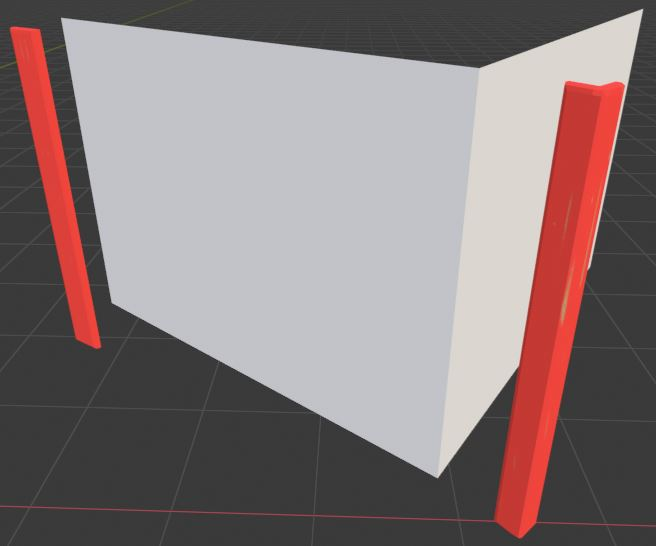
\includegraphics[width=0.35\textwidth]{bilder/holzecke2}
      \caption{Überarbeitete Wandelemente und Holzbalken aus neuem Subkit.}\label{holzecke2}
          \vspace{-14pt}
\end{wrapfigure}
Die zuvor in die Wände eingesetzten Holzbalken wurden wieder von den Wänden gelöst und wurden in ein eigenes Subkit verschoben. In diesem Subkit gibt es Holzbalken für die verschiedenen hohen Module und auch für Außen- und Innenecken. Durch diese Änderungen wurden die Probleme mit den Schatten gelöst. Zusätzlich können so verschiedene Versionen von Holzbalken genutzt werden, wodurch eine sichtbare Wiederholung vermindert wird. Auch ist es möglich Wände ohne Holzbalken zu bilden, was weitere Möglichkeiten eröffnet.
\newpage
Nach diesen Anpassungen wurden weitere Tests durchgeführt. Bei diesen wurde festgestellt, dass bei einer bestimmten Kombination von Dach- und Balkonelementen im Dach Lücken entstehen können, die nicht mit bestehenden Modulen gefüllt werden können. Die Lücken hatten eine Breite von 1,28 Metern, dies entspricht einem Viertel der normalen Breite aller Elemente.
\par
\begin{wrapfigure}{l}{0.4\textwidth}
  \centering 
   \vspace{-12.5pt}
    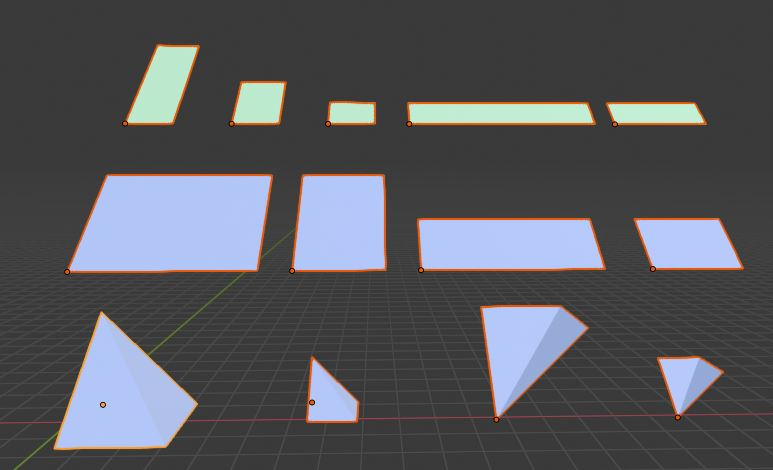
\includegraphics[width=0.4\textwidth]{bilder/DacheElemente}
      \caption{Ursprüngliches Elemente für den Abschluss des Daches (blau) und neue Elemente für das schließen spezifischer Lücken (grün).}\label{DacheElemente}
          \vspace{-14pt}
\end{wrapfigure}
Nach mehreren erfolglosen Versuchen diese Lücken, ohne viele neue Elemente zu vermeiden, wurde dem Subkit, für die Schließung des Gebäudes, weitere Elemente hinzugefügt. Auf Basis der bestehenden Elemente wurden neue Elemente in verschiedenen Kombinationen aus einem Viertel der Höhe und einem Viertel der Breite erstellt.
\par
Mit diesen neuen Modulen war das Kit vollständig (Abbildung \ref{finalmodul}) und alle Modelle konnten weiter ausgearbeitet werden.
\begin{figure}[H]
\centering
  \makebox[\textwidth]{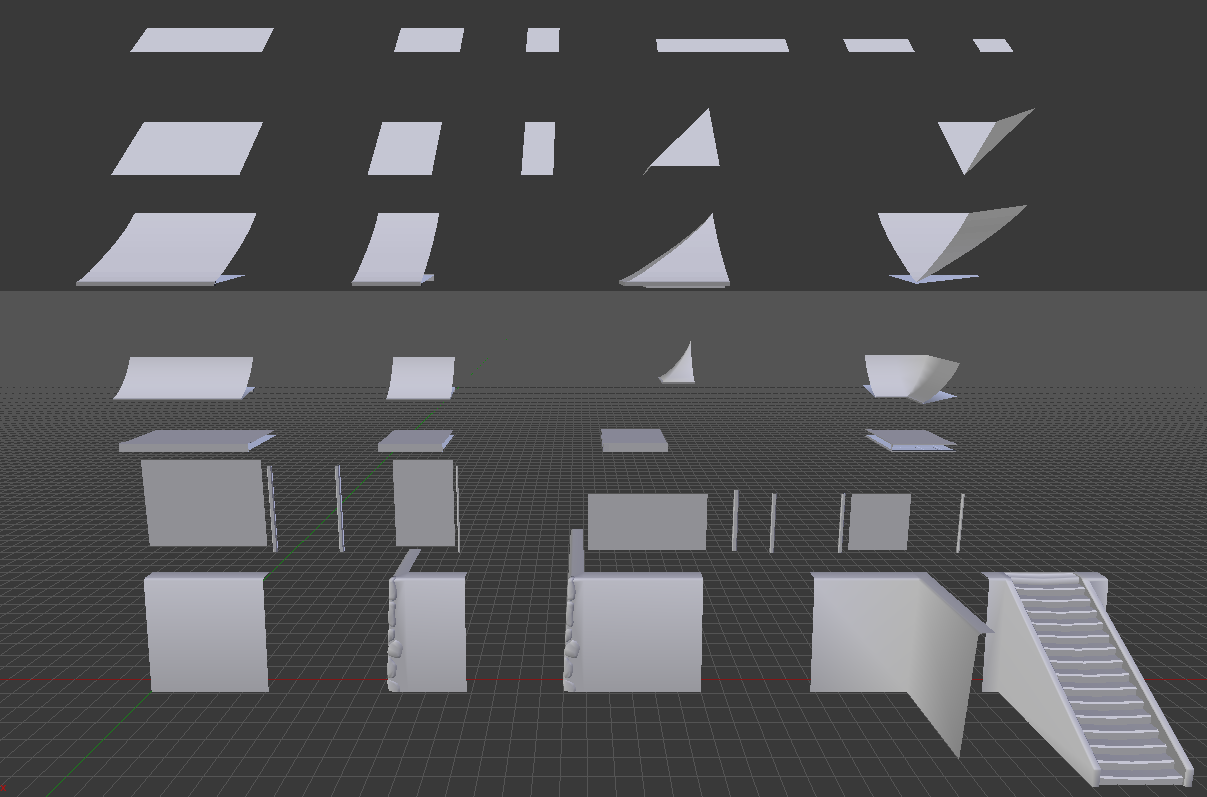
\includegraphics[width=1\linewidth]{bilder/Prototypen2}}
  \caption{Prototypen des weiterentwickelten Systems.}
	\label{finalmodul}
\end{figure}
\vspace{-10.5pt}
Die finalen Module wurden von unten nach oben entwickelt. Zuerst wurde das Fundament fertiggestellt, dann die Wände, die Vordächer, die Balkone und zum Schluss die Dachelemente, die das Gebäude abschließen. Auf diese Weise konnte immer überprüft werden, ob die neuen Elemente ohne Probleme auf die unterliegende Schicht passen.
\par
Aufgrund der speziellen Architektur der Gebäude konnte keine vollständige Modularität erreicht werden. Module sind horizontal immer nur mit Modulen des gleichen Subkits kombinierbar. Vertikal können alle Subkits miteinander verbunden werden. Ausschließlich das Fundament-Subkit kann nur als unterste Ebene fungieren, da es auf Grund seiner speziellen Form nicht auf andere Elemente gesetzt werden kann.
\begin{figure}[H]
\centering
  \makebox[\textwidth]{\includegraphics[width=1\linewidth]{bilder/AllModules}}
  \caption{Alle Module mit angewandten Texturen.}
	\label{alleModule}
\end{figure}
\vspace{-10.5pt}
Für das Projekt wurden insgesamt 76 verschiedene Elemente erzeugt. Von den Wand-, Balkon- und Holzbalkenelementen wurden zusätzliche Varianten erzeugt, um eine abwechslungsreichere Gestaltung zu ermöglichen. Zusammen mit diesen entstanden insgesamt 126 Module. Abbildung \ref{alleModule}, zeigt alle erstellten Module in ihrem finalen Zustand.
\newpage
\section{Texturierung}
Wie zuvor erwähnt, steht in dieser Arbeit die Erstellung der Modelle im Vordergrund; infolgedessen wird in diesem Abschnitt nur skizziert, wie für die Texturierung vorgegangen wurde.
\par
Nach der Planungsphase wurde für alle benötigten Texturen eine Vorabversion erstellt. So konnten für die Modelle schon passende UV-Maps erstellt werden. Hier war zu beachten, dass die Ränder der Modelle mit den Rändern der Textur verbunden wurden. Nur so kann ein nahtloser Übergang zwischen Modulen gewährleistet werden. Durch das Texturieren der Modelle konnte schon früh ein Eindruck vermittelt werden, wie die Module später aussehen werden. Die finale Version der Texturen wurde nach Abschluss der Modellierphase erstellt.
\par
Um zu erfahren, welche verschiedenen Texturen benötigt werden, wurden Bilder der nachzubildenden Gebäude auf genutzte Baumaterialien hin analysiert. Zusammen mit dem vorliegenden Konzept (Abblidung \ref{JapanKonzept}) konnte so eine Liste mit benötigten Texturen ausgearbeitet werden.
\begin{figure}[H]
\centering
  \subfloat[][Steintextur für Fundamentelemente.]{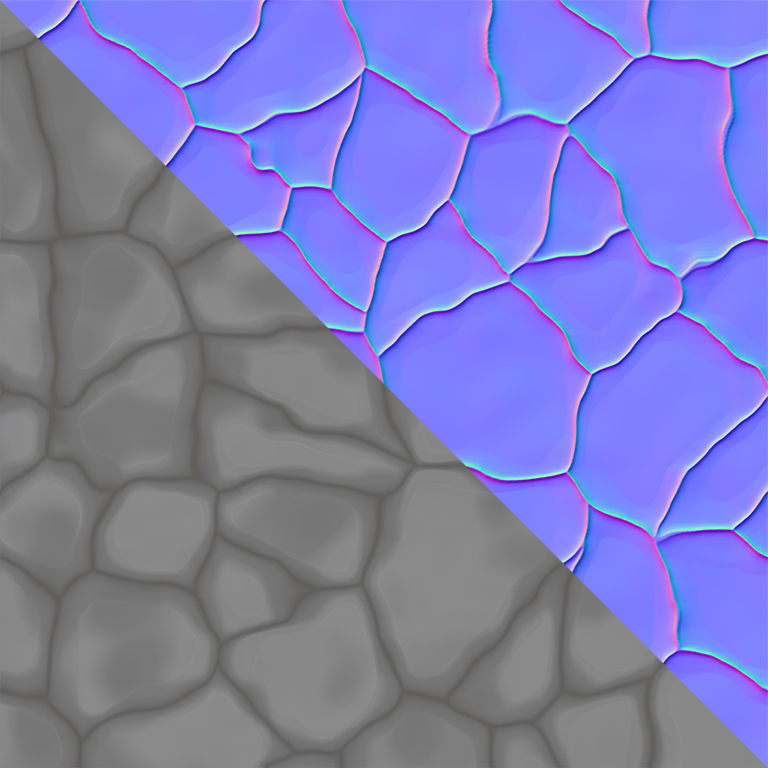
\includegraphics[width=0.29\linewidth]{bilder/StoneWall}\label{StoneWall}}%
  \qquad
  \subfloat[][Steintextur für Treppenstufen.]{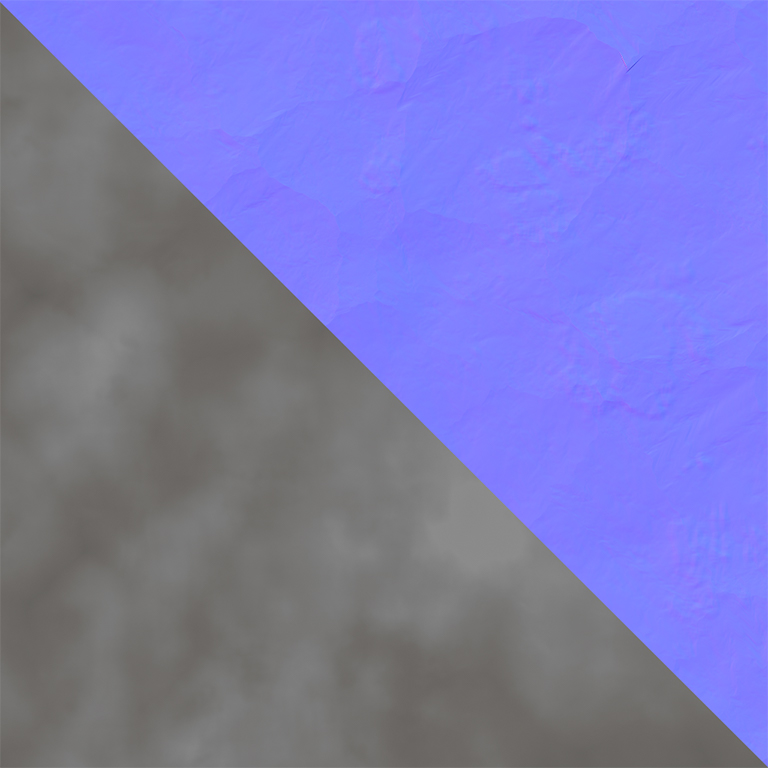
\includegraphics[width=0.29\linewidth]{bilder/StoneStairs}\label{StoneStairs}}%
   \qquad
  \subfloat[][Dachziegeltextur für Dachelemente.]{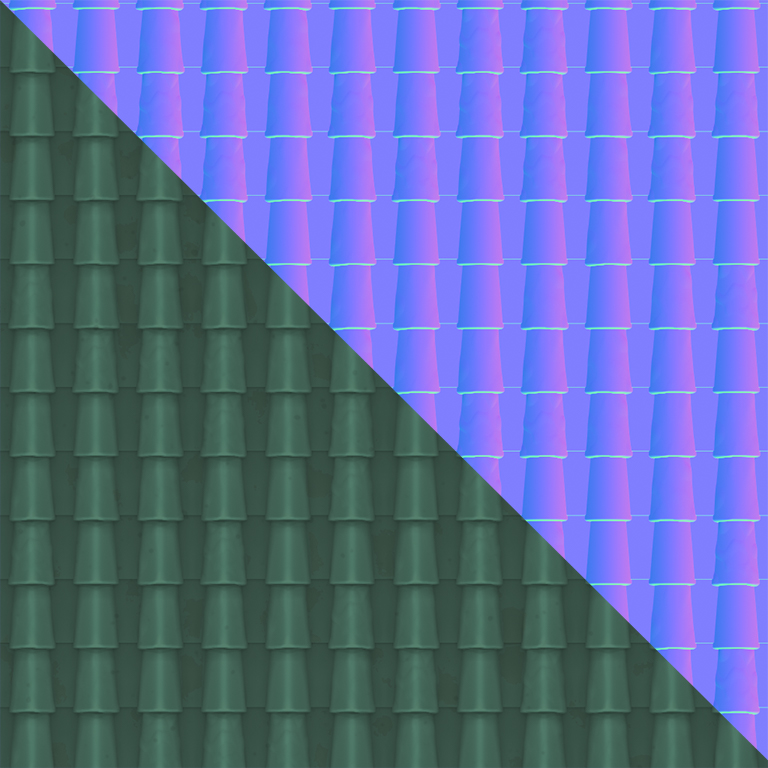
\includegraphics[width=0.29\linewidth]{bilder/RoofTiles}\label{RoofTiles}}%
   \qquad
  \subfloat[][Holztexturen für Holzelemente.]{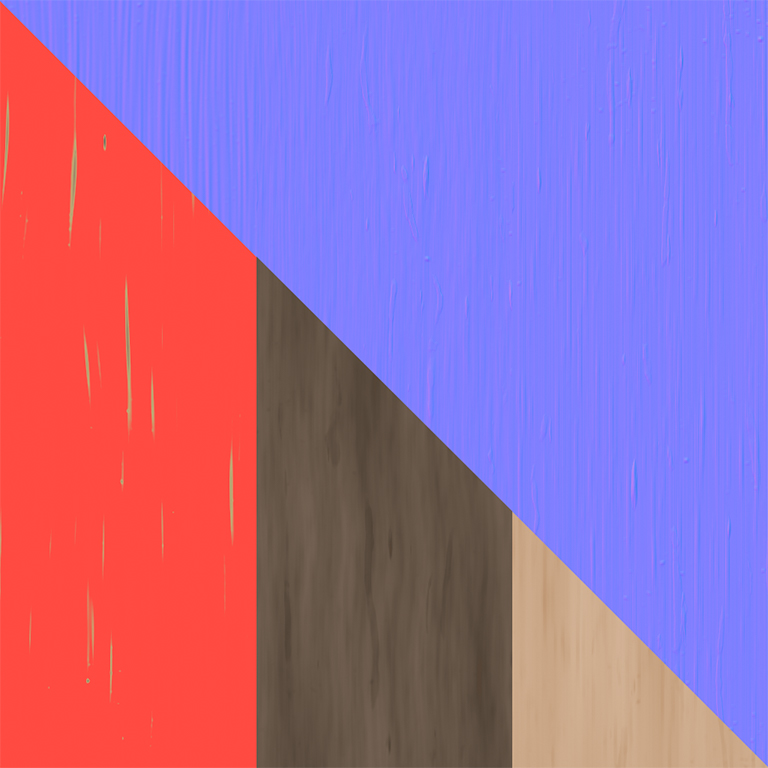
\includegraphics[width=0.29\linewidth]{bilder/Wood}\label{Wood}}%
   \qquad
  \subfloat[][Steintextur für Wandelemente.]{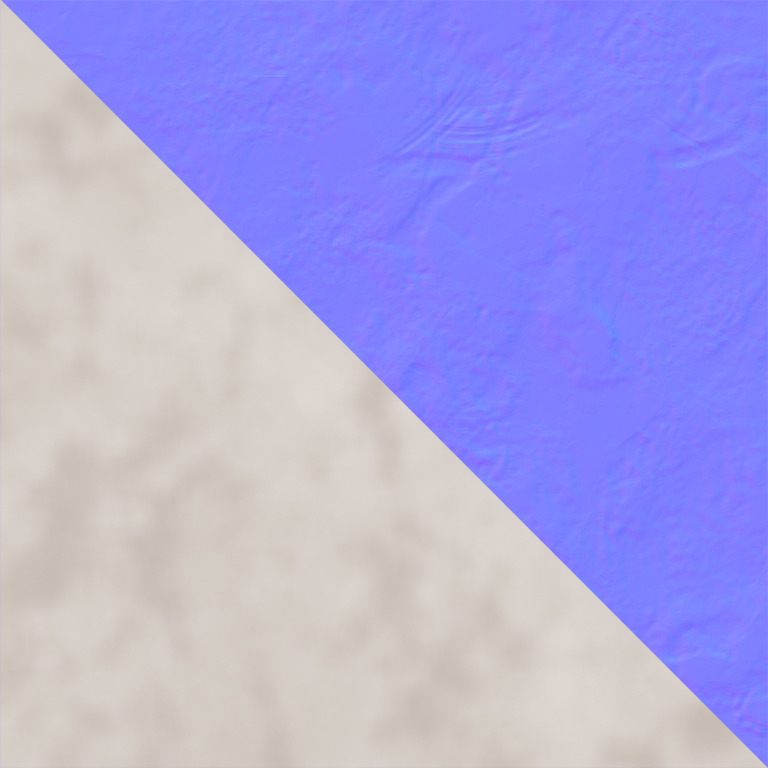
\includegraphics[width=0.29\linewidth]{bilder/WhiteWall}\label{WhiteWall}}%
   \qquad
  \subfloat[][Papiertextur für Fenster.]{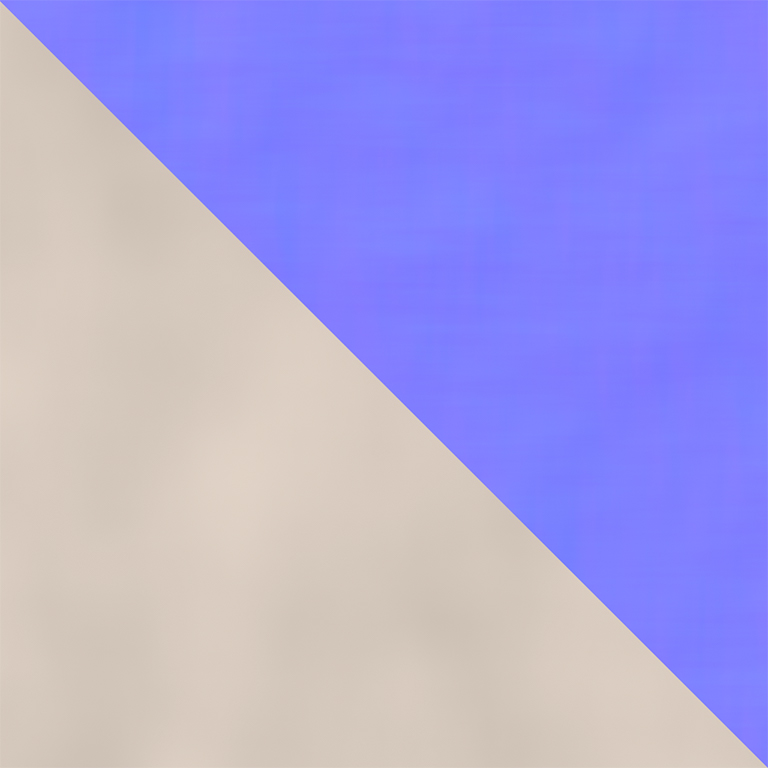
\includegraphics[width=0.295\linewidth]{bilder/Paper}\label{Paper}}%
  \caption{Ausschnitte aller benötigten Diffuse- und Normalmaps.}%
\label{Textures}
\end{figure}
\vspace{-10.5pt}
Im Anschluss wurden alle Texturen mit \textit{Substance Designer} erstellt. Werden Texturen mit den Standardeinstellungen von \textit{Substance Designer} erstellt, sind diese immer so ausgelegt, dass sie in alle Richtungen kachelbar sind. Diesbezüglich mussten also kein spezielles Vorgehen beachtet werden.
\begin{figure}[H]
\centering
  \subfloat[][Specularmap.]{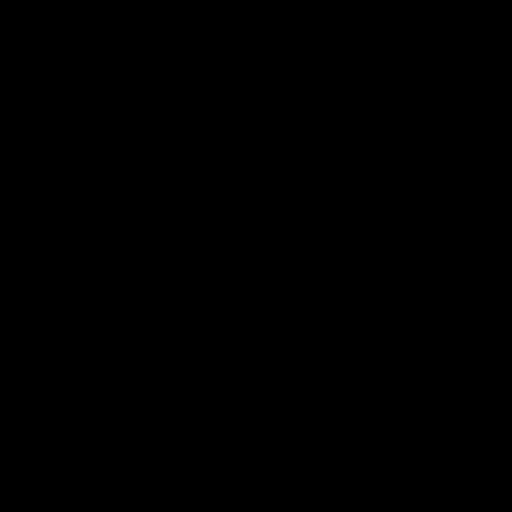
\includegraphics[width=0.34\linewidth]{bilder/specular}\label{specular}}%
  \qquad
  \subfloat[][Rougnessmap.]{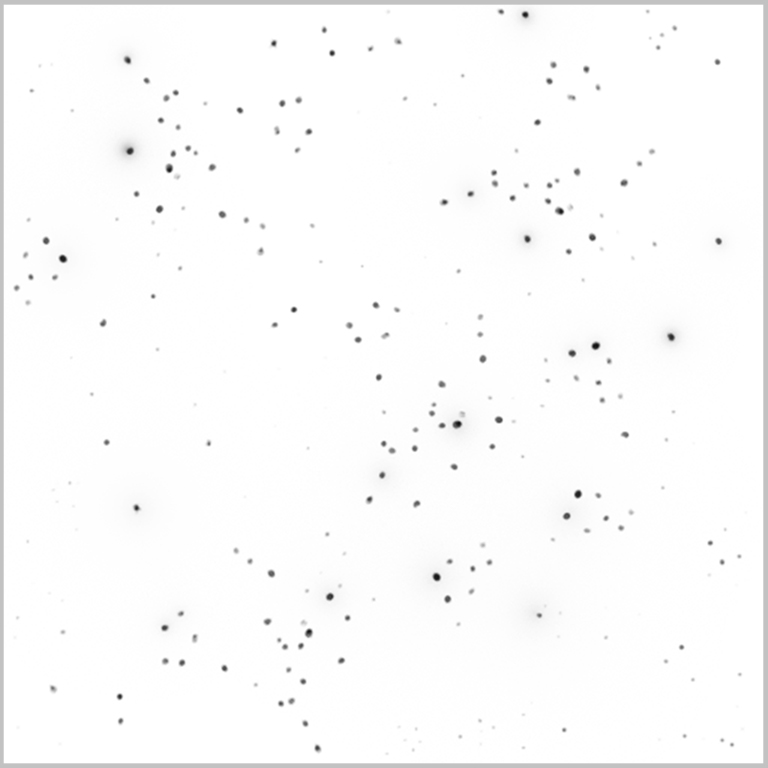
\includegraphics[width=0.34\linewidth]{bilder/roughness}\label{roughness}}%
  \caption{Die für die meisten Modelle genutzten Rougness- und Specularmaps.}%
\label{altemaps}
\end{figure}
\vspace{-10.5pt}
In \textit{Renegade Line} werden für die Materialien Albedo-, Normal-, Roughness- und Specularmaps genutzt. Die Roughness- und Specularmap werden von den bestehenden Modellen übernommen. Diese sind größtenteils einfarbig und sorgen für ein eher stumpfes Erscheinungsbild der Modelle. Dies ist für den angestrebten Cartoon Look sehr wichtig. Die Albedo- und Normalmap wurde für jede Textur von Grund auf neu erzeugt. Für die Griffe an den Türen wurde ein schon existierendes Metall Material genutzt.
\begin{figure}[H]
\centering
  \makebox[\textwidth]{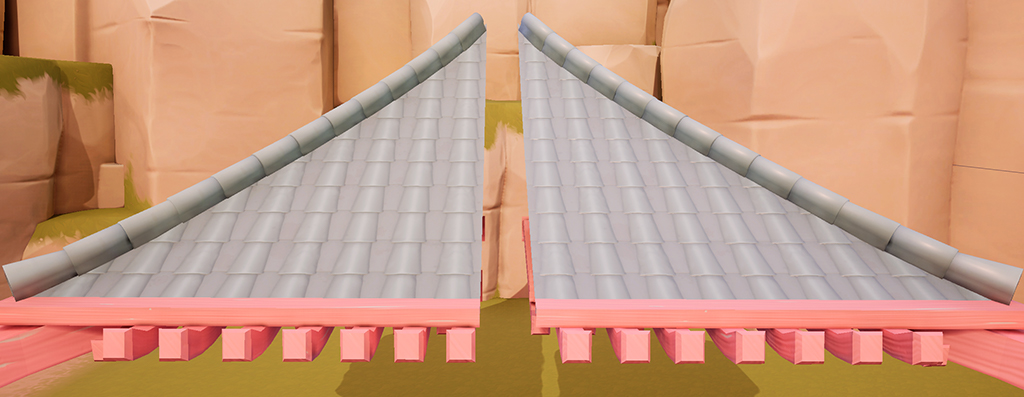
\includegraphics[width=\linewidth]{bilder/specroughvs}}
  \caption{Einfluss der Specular- und Roughnessmap (links) im Vergleich mit den Standartwerten aus UE (rechts).}
	\label{specroughvs}
\end{figure}
\vspace{-10.5pt}
Von den Holztexturen für Holzbalken und Leisten an Türen, Fenstern und Dächern wurden drei Versionen erstellt: Eine, zum Konzept passende Rote sowie eine mit hellem und eine mit dunklem Holz (Abbildung \ref{Wood}). So kann ein Gebäude durch Tausch einer Textur einen ganz neuen Look erhalten.
\par
Versuche einen Texturatlas zu nutzen wurden nach Tests in UE nicht weiter verfolgt. Durch Mip Mapping, ein Vorgang bei dem Texturen komprimiert werden, um eine bessere Spielperformance zu gewährleisten, wurden nebeneinander liegende Texturen vermischt. Diese Vermischung führte zu sichtbaren Kanten auf den Modellen. Zusätzlich wäre es komplizierter gewesen die verschiedenen Holzarten zu nutzen, wenn diese nicht in verschiedene Materialien aufgeteilt worden wären.
\section{Implementierung}\label{implementierung2}
Nachdem alle Tests bezüglich der Funktion und des Aussehens des Kits abgeschlossen waren, wurden alle Testdateien aus dem UE-Projekt entfernt.
\par
Im Anschluss wurden für Texturen, Materialien, Modelle und fertige Gebäude Ordner angelegt. Der Ordner für die Modelle wurde mit Unterordnern für die Subkits gefüllt. Die fertigen Modelle sollten in Blueprints\footnote{\,In Unreal Engine sind Blueprints eine Art leerer Container der Code ausführen und Objekte enthalten kann.} abgespeichert und in dem dafür vorgesehenen Ordner gesichert werden.
\par
Zuerst wurden alle Texturen importiert und auf deren Grundlage neue Materialien erstellt. Dann wurden die Modelle importiert und jedem Modell wurde ein Standardset an Materialien zugeordnet. Alle Modelle mit Holzelementen wurden mit dem roten Holz ausgestattet, dessen Verwendung als Preset vorgesehen ist.
\par
Nach der Implementierung wurden für  Tests erste Gebäude in UE erstellt. Die schon zuvor festgestellten Belichtungsprobleme an glatten Übergängen konnten durch Anpassungen der Lichtberechnung in den Welteinstellungen und dem Vergrößern der Lightmap gelöst werden. Die Lightmap ist ein Bild in der die Schattenwerte gespeichert werden, die durch die Berechnung des Lichtes ermittelt wurden. Die Modelle nutzen nun eine Lightmap-Größe von 128 x 128 Pixeln. Die vorkonfigurierten 64 x 64 Pixel waren zu klein und führten an manchen Stellen zu Überlappungen zwischen den Faces.
\begin{figure}[H]
\centering
  \makebox[\textwidth]{\includegraphics[width=\linewidth]{bilder/LichtProblem}}
  \caption{Harte Kanten an Modulübergängen von Modulen.}
	\label{LichtProblem}
\end{figure}
\vspace{-10.5pt}
Das Ändern der Lichtberechnungseinstellungen verlangsamte die Lichtberechnung. Da dieser Prozess vor dem Spielen ausgeführt wird, hat dies keinen negativen Einfluss auf die Spielperformance, erhöht aber die Dauer von Tests in der Entwicklung. Nachdem die Probleme der Beleuchtung gelöst waren, wurden weitere Gebäude erstellt.
\newpage
Während dessen wurden keine Probleme festgestellt. Alle Module konnten wie geplant ohne Fehler verbunden werden. So wurden zehn verschiedene Gebäude erstellt, um mögliche Formen und Größen der Gebäude zu testen. Um zu überprüfen, ob sie beziehungsweise das modulare Kit in die alte Spielwelt passen, wurden die Gebäude in ein bestehendes Level eingefügt.
\begin{figure}[H]
\centering
  \makebox[\textwidth]{\includegraphics[width=\linewidth]{bilder/StilTest}}
  \caption{Aus dem Kit erstellte Gebäude in einem alten Level.}
	\label{stilTest}
\end{figure}
\vspace{-10.5pt}
Die neuen Gebäude fügen sich sehr gut in den bestehenden Spielstil ein, auch wenn die übrigen Assets ein anderes Setting repräsentieren. Das an dem Spiel beteiligte Team war sich über die Diskussion der Ästetik hinaus einig, dass die neuen Gebäude zu dem bestehenden Stil passen.
\par
Der praktische Teil der Arbeit ist hier beendet, im Folgenden werden die Ergebnisse dieses Projektes zusammengefasst und ausgewertet.
\chapter{Evaluation}
\section{Kit}
In diesem Abschnitt wird das unter Anwendung der erarbeiteten Methoden entstandene modulare Kit bewertet.
\par\textbf{Performance}\par
Für eine bessere Bewertung des Kits wurde ein Performance-Test durchgeführt, der ernüchternde Ergebnisse lieferte.
\par
Die Tests wurden auf einem sehr leistungsstarken Desktop-PC\footnote{\,Der PC ist aus folgenden Komponenten zusammengesetzt: INTEL CORE i7-4790K 4.0GHz, GeForce GTX 970 4GB Grafikkarte, 16GB Arbeitsspeicher und 1TB HDD Festplatte.} durchgeführt. 
\par
Es wurden zwei verschiedene Gebäude in zwei Versionen für die Tests genutzt: Jeweils eine, aus Modulen in UE zusammengesetzte Version und eine, die in Blender erstellt und als ein einzelnes Objekt in UE importiert wurde. Ein Gebäude ist einfach aufgebaut und soll vielfach in einem Level auftauchen. Während des Spielens sieht der Spieler ungefähr zehn der einfach aufgebauten Gebäude auf einmal, diese Zahl kann je nach Level und Position des Spielers variieren. Das andere Gebäude ist größer und komplexer aufgebaut, es repräsentiert eine Art Palast der pro Level nur einmal vorkommen soll.
\par
Die Komplexität der Modelle lässt sich wie folgt darstellen:
\begin{table}[H]
\fontsize{9}{10}\selectfont
\begin{tabular}{ p{0.094\textwidth} |  p{0.407\textwidth} |  p{0.407\textwidth} }
\vspace{74pt}Kleines \newline Gebäude &
\vspace{0.2pt}
\includegraphics[width=\linewidth]{bilder/smallhousepiece}\newline
26.000 Triangles, 7  Materialien &
\vspace{0.2pt}
\includegraphics[width=\linewidth]{bilder/smallhousemodular}\newline
40 Module\\ \hline
\vspace{97pt}Großes \newline Gebäude&

\vspace{0.2pt}\includegraphics[width=\linewidth]{bilder/castleonepiece}\newline
155.000 Triangles, 8 Materialien &

\vspace{0.2pt}\includegraphics[width=\linewidth]{bilder/castlemodular}\newline
 342 Module\\ \hline
& 
\vspace{0.2pt}
Normale Ausführung &
\vspace{0.2pt}
Modulare Ausführung
\end{tabular}
 \caption{Aufbau und Eigenschaften der für die Performance-Test genutzten Gebäude.}
\end{table}
\newpage
Für die Tests wurde ein leeres Level erstellt, in das eine Bodenebene und ein direktionales Licht eingefügt wurde. Mit Hilfe von Blueprints wurde das Level mit verschieden viel Gebäuden einer Art gefüllt. Nach Berechnung des Lichts wurden im Playmode verschiedene Werte gemessen. Der Test konnte auf der verwendeten Hardware mit 500 der großen Gebäude nicht durchgeführt werden.
\begin{figure}[H]
\centering
  \makebox[\textwidth]{\includegraphics[width=\linewidth]{bilder/PerformancteTestFPS}}
  \caption{Übersicht der Bildfrequenzen aus den durchgeführten Tests.}
	\label{PerformancteTestFPS}
\end{figure}
\begin{figure}[H]
\centering
  \makebox[\textwidth]{\includegraphics[width=\linewidth]{bilder/PerformancteTestDC}}
  \caption{Übersicht benötigter Draw Calls  aus den durchgeführten Tests.}
	\label{PerformancteTestDC}
\end{figure}
\newpage
Die Diagramme (Abbildung \ref{PerformancteTestFPS} und \ref{PerformancteTestDC}) zeigen, dass die Performance der nicht-modularen Gebäude deutlich besser ist. Die nötigen Draw Calls und die resultierende Last auf das System sind für die modularen Gebäude um ein Vielfaches höher als bei den nichtmodularen Gebäuden. Auch die Bildwiederholungsrate ist bei den klassischen Gebäuden bedeutend höher.
\par
Nach den Tests wurde versucht, die Performance der modularen Elemente zu verbessern. Das in Abschnitt \ref{Implementierung1} beschriebene \textit{Instancing} wird von der genutzten Version 4.21 von UE nur teilweise automatisch angewendet. Die Modelle werden nur einmal in den Speicher geladen, aber jedes Modell erzeugt für sich und seine Materialien eigene Draw Calls.
\par
Mit Hilfe des Tools \enquote{AutoInstance}\footnote{\,Das Tool kann unter: \url{https://www.unrealengine.com/marketplace/en-US/slug/auto-instance} abgerufen werden.} aus dem Unreal Engine Marketplace wurde versucht das Instancing der Module zu verbessern.
\par
Das Tool konnte die Draw Calls drastisch verringern. Trotzdem konnte die Performance nicht verbessert werden, da durch das \textit{Instancing} an anderer Stelle neue Last entstand. Zudem wurde die Zuweisung der Materialien durch das Instanziieren der Module verändert und konnte nicht mehr angepasst werden.
\par
Die Instanziierung des Tools kann auch manuell durchgeführt werden, jedoch würde dies zu unverhältnismäßig viel Arbeit führen und müsste für jedes Level neu durchgeführt werden.
\par
In UE können mehrere Objekte zu einem verbunden werden. Bei Tests dieser Funktion zeigte sich, dass bei der Verbindung von Modulen alle Material Slots erhalten bleiben. Dies hat zur Folge, dass wieder mehr Draw Calls erzeugt werden, als wenn das Gebäude in einem Stück in UE importiert werden würde. Das große Gebäude aus dem Performance-Test hatte nach dem Verbinden in der Engine 737 zugewiesene Materialien anstelle von 8.
\par
Da die Performance-Unterschiede auch schon bei einer für das Spiel normalen bis geringen Anzahl von gleichzeitig sichtbaren Gebäude deutlich waren und es zu diesem Zeitpunkt keine Lösung gab, dies zu ändern, wurde davon abgesehen, das Kit in UE zu nutzen.
\par
Die schon in UE erstellten Gebäude wurden in Blender nachgebaut und in UE importiert.
\par
Da nach den Tests in UE normale Modelle genutzt werden, ist der Einfluss auf die Performance identisch mit dem von normal erstellten Assets.
\par\textbf{Visuelle Qualität}\par
Gebäude, die mit dem neuen Kit erstellt wurden, erreichen das gleiche Level an Detail und Qualität, wie die schon bestehenden Assets und fügen sich sehr gut in den Spielstil ein.
\newpage
Tests bezüglich der Kunstermüdung (siehe Abschnitt \ref{vqualitaet}) können aufgrund von fehlender Assets für ein gesamtes Level und der begrenzten Zeit nicht durchgeführt werden. Alle bisherigen Level wurden auf der Basis von neun Gebäuden erstellt. Mit dem modularen Set können weit mehr als neun verschiedene Gebäude erstellt werden. Das Nutzen des Kits sollte demnach keinen negativen Effekt auf das optische Erscheinungsbild des Levels haben.
\par
Durch weitere Varianten der Dachmodule könnte das Kit noch verbessert werden. Die Dächer aller Gebäude sehen gleich aus, auch wenn sie andere Formen haben.
\par
Durch das Zusammensetzen der Module in Blender kann jedes Modell, neben dem Kombinieren verschiedener Module, auch mit einem individuellen Look versehen werden, indem das erstellte Gebäude durch Modifikationen der Meshes abgeändert wird. Hierdurch lässt sich die Qualität der Module weiter erhöhen, es wird aber auch weitere Arbeitszeit benötigt.	
\par
Die von Burgess und Purkeypile erwähnte Boxartigkeit von modularen Assets ist auch in diesem Set zu erkennen. Dies ist jedoch zum Teil auf die Bauweise der Gebäude zurückzuführen, welche durch das Kit abgebildet werden sollten und fällt in diesem Fall nicht negativ auf.
\par\textbf{Nutzerfreundlichkeit}\par
Die Nutzerfreundlichkeit des Kits sollte durch einen Level-Designer geprüft werden. Da die Modelle nach dem Performance-Test in Blender vorgefertigt werden müssen, wäre das Erstellen von Gebäuden in der Engine durch den Level-Designer überflüssige Arbeit und wurde ausgelassen. Durch die durchgeführten Tests und die dadurch entstandenen Gebäude, wurde dennoch ein guter Eindruck der Handhabung vermittelt.
\par
Gebäude von kleiner bis mittlerer Größe lassen sich schnell erstellen. Steigt die Größe des Gebäudes weiter an, erhöht sich die benötigte Zeit jedoch drastisch. Für größere Gebäude wäre es von Vorteil, wenn das Kit größere Elemente besitzen würde. Da aber hauptsächlich kleine bis mittlere Gebäude erstellt werden sollen, fällt dies nur gering negativ auf.
\par
Da in Blender die gleichen Methoden wie in UE genutzt werden können und zusätzlich weitere Methoden zur Verfügung stehen, wurde die Nutzerfreundlichkeit in diesem Aspekt noch verbessert.
\par\textbf{Aufwand}\par     
Das Erstellen der Assets hat viel Zeit gekostet. Vor allem zu Beginn war es schwierig das Konzept der Modularität zu greifen und die Gebäude richtig in passende Module aufzuteilen. Hierfür wurde die meiste Zeit der Planung aufgebracht.
\par
Nur für das eine Level wäre es vermutlich schneller gewesen, einzelne Gebäude zu erstellen. Werden noch weitere Level in dem gleichen Setting entwickelt, kann der Arbeitsaufwand wohl ausgeglichen werden.
\newpage
Könnte das Kit, wie geplant, in UE genutzt werden, hätte die benötigte Arbeitszeit, um Gebäude zu erstellen, besser auf das Team verteilt werden können. Das Erstellen und Anpassen der Gebäude aus den vorgefertigten Modulen wäre von den Level-Designern übernommen worden. So wäre es möglich gewesen, dass der 3D-Artist ohne Unterbrechungen an weiteren Assets für das Level arbeitet.
\par
Durch das Vorbauen der Modelle in Blender kann die Aussage von L. Durand  bezüglich der leichten und schnellen Anpassung der Gebäude auf das Gameplay nicht überprüft werden.
\par
Die Bewertung des Kits ist hier beendet. Im Folgenden wird zuerst darauf eingegangen, welche der zuvor erarbeiteten Methoden im Verlaufe des Projektes angewandt wurden und welchen Nutzen diese hatten.
\section{Methoden}
\par\textbf{Raster}\par
Ohne die Nutzung eines Rasters wäre das passgenaue Platzieren der Module so zeitaufwändig gewesen, dass es keinen Sinn ergeben würde ein modulares Kit zu nutzen.
\par
Auch bei der Erstellung der Module hat das Raster eine entscheidende Rolle gespielt. Ohne Anhaltspunkte, die durch das Raster gegeben waren, wäre es sehr schwer gewesen, ein modulares System zu entwickeln, durch welches alle Teile miteinander verbunden werden können.
\par
Die von Burgess und Purkeypile erwähnte Methode, das Raster zu verlassen (siehe Abschnitt \ref{weitereT}) und an vorher platzierten Objekten auszurichten, wurde nicht genutzt. Dies hätte die Erstellung vieler neuer Module und Modifikationen  des Kits gefordert. Die Bauweise der nachzubildenden Gebäude bedient sich in der Regel nur an rechten Winkeln, welche mit dem Kit dargestellt werden können. Es gab also auch keinen Grund diese Methode zu nutzen.
\par\textbf{Pivot Point}\par
Nur durch die richtige Platzierung des Pivot Points konnte das volle Potenzial des Rasters genutzt werden. Für die Positionierung des Pivot Points wurden die Regeln\footnote{\,Eine Übersicht der Regeln kann in einem \textit{Gamasutra}-Artikel \parencite{Mader} von P. Mader unter dem Abschnitt \textit{Pivot Placement} gefunden werden.} von P. Mader genutzt. Diese waren sehr leicht anzuwenden und hilfreich, um eine praktische Position für Pivot Points zu finden.
\par
Sein Hinweis darauf den Pivot Point bei Objekten, die einen Kreis formen, in das Zentrum des Kreises zu setzen, wurde für dieses Objekt auch bei Eckmodulen angewandt. Dies beschleunigt die Neupositionierung und Ausrichtung dieser Elemente.
\newpage
\textbf{Textur}\par
Der Einsatz von kachelbaren Texturen war für das Kit unabdinglich. Darüber hinaus musste nicht viel beachtet werden außer, dass in der UV-Map die Ränder der Modelle mit den Rändern der Textur verbunden werden. Nur so war gewährleistet, dass keine sichtbaren Kanten zwischen den Modulen entstehen, die den Eindruck stören würden, dass die Gebäude aus einem Stück bestehen.
\par\textbf{Planung und Tests}\par
Ein weiterer wichtiger Aspekt des Projektes war das Planen und Testen. Auch wenn dies keine praktisch anwendbaren Methoden sind, wie die anderen hier aufgelisteten, sind sie nicht weniger wichtig.
\par
Ohne die vorherige Planung und diverse Tests, hätte die Entwicklung des Kits mehr Zeit in Anspruch genommen und hätte vermutlich keine so hohe Qualität erreicht.
\par
Mit der gewonnenen Erfahrung kann die Planungsphase bei einem nachfolgenden Projekt voraussichtlich schneller und besser durchgeführt werden. Viele der nötigen Änderungen am Kit hätten durch mehr Praxiserfahrung schon in der ersten Planungsphase erkannt werden können, was den generellen Ablauf des Projektes beschleunigt hätte.
\par
Auf Tests und eventuelle Weiterentwicklungen des Kits sollte dennoch nicht verzichtet werden. Die in der Planungsphase erstellten Regeln sollten angepasst werden, wenn dadurch das Kit verbessert wird, auch wenn dadurch mehr Arbeit entsteht. Je nach Projekt wird das Kit an vielen Stellen und für lange Zeit genutzt und sollte daher so gut wie möglich ausgearbeitet sein.
\par\textbf{Varianten}\par
Die Subkits bestehen aus allen nötigen Teilen, um verschiedene Gebäude zu bauen. Diese hätten alle ein sehr ähnliches Erscheinungsbild, wenn das Kit keine Varianten der Module enthalten würde. Bisher wurden nur von den Wand-, Balkon- und Holzbalkenelementen Varianten erstellt. Nur durch diese lassen sich schon viele individuell aussehende Gebäude erzeugen. Die Erzeugung weiterer Varianten nimmt nur wenig Zeit in Anspruch, da von einem Basis Modell aus gearbeitet werden kann, welches schon an die Regeln des Kits angepasst wurde.
\par
Das Nutzen von Varianten ist also ein effizienter Weg ein Kit zu ergänzen.
\par
\textbf{Modularitätsstufen}\par
In diesem Projekt wurde eine mittlere bis kleine Stufe der Modularität gewählt. Folglich ist es möglich mit einer kleinen Auswahl an Modulen viele verschiedene Objekte zu erstellen. Würde ein Gebäude aus nur drei Modulen bestehen, müssten viel mehr Module erstellt werden, um die gleiche Abwechslung zu gewährleisten.
\par
Wie schon erwähnt wurde die Spielperformance durch die vielen genutzten Elemente negativ beeinflusst. Die Lösung, die Gebäude in Blender vorzufertigen, verringert nicht die positiven Aspekte der gewählten Stufe, da diese auch in Blender genutzt werden können.  
\par\textbf{Benennung}\par
Eine gut konzipierte Benennung der Module ist, wie von Burgess und Purkeypile angeführt, ein sehr wichtiger Aspekt, um Arbeitsabläufe mit dem Kit zu beschleunigen und die Kommunikation zu verbessern. Wie zuvor beschrieben, muss darauf geachtet werden, eine sinnvolle Bezeichnung der Module zu entwickeln, die leicht zu interpretieren und zu erlernen ist. Sind bei Tests Probleme mit Modulen aufgefallen, konnten diese leicht durch ihren Namen zugeordnet werden.
\par\textbf{Struktur}\par
Zusammen mit der Benennung war das Einführen einer Ordnerstruktur sehr hilfreich, um den Prozess der Gebäudeerstellung in UE zu beschleunigen. Auch wenn dies nur zu einem gewissen Grad getestet wurde. Des Weiteren konnte durch das Einteilen der Module in Subkits der Erstellungsprozess besser organisiert und die Übersicht in UE dadurch deutlich verbessert werden.
\par\textbf{Vertex Farben}\par
Das Einfärben von Vertices, um die Erscheinung der Texturen bzw. die des Models zu verändern, wurde nicht angewandt. Hierfür hätten weitere Module erstellt werden müssen. Da das Kit auch ohne diese Methode schon genug Abwechslung aufwies, wurde darauf verzichtet. Aufgrund des veränderten Arbeitsablaufes könnte dies ohne großen Aufwand für neue Gebäude genutzt werden, um mehr Abwechslung zu schaffen ohne neue Module zu entwickeln.
\chapter{Fazit und Ausblick}
\section{Fazit}
Durch das Aufzeigen des Einflusses von Modularität auf die Entwicklung von Videospielen und die Realität, konnte ein erster Eindruck von dessen Nutzen gewonnen werden. Zudem wurde dargelegt, das dieses Prinzip schon lange angewandt wird und stetig weiterentwickelt wird. Die Erarbeitung des normalen Ablaufs der Asseterstellung und wie dieser durch spezielle Methoden auf die Anwendung von modularem Design angepasst wird, hat gezeigt, welche Tiefe dieses Konzept besitzt. Durch die Anwendung der Methoden und Konzepte konnten diese bewertet und eine Einschätzung von modularem Design erstellt werden.
\par
Eine ausführliche Bewertung der genutzten Methoden wurde schon im vorherigen Kapitel durchgeführt. Zusammenfassend lässt sich sagen, dass die wichtigsten Methoden, um modulares Design zu realisieren, die folgenden sind:
\begin{itemize}
\item Raster,
\item Pivot Point,
\item Planung,
\item Tests und
\item kachelbare Texturen.
\end{itemize}
Alle weiteren Methoden verbessern den Prozess, aber ohne die zuvor genannten, ist die praktische Umsetzung eines modularen Kits nicht möglich. Für andere Ansätze von Modularität kann diese Bewertung abweichen.
\par
Durch die vielen schon vorhandenen Methoden, welche trotz ihres Alters alle noch relevant sind und meist gut miteinander funktionieren, ist es leicht einen Einstieg in modulares Design zu finden. Ohne viel Zeit in die gründliche Planung zu investieren, lässt sich das Konzept jedoch nur schwer umsetzen.
\par
Auf Grund dieser großen Zeitinvestition vorab, muss für jedes Projekt geprüft werden, bis zu welchem Grad es sinnvoll ist Modularität zu nutzen. Lassen sich Assets nicht wieder verwerten oder wird immer nur eine geringe Anzahl ähnlicher Objekte genutzt, sollte von einem modularen Kit abgesehen werden. Dennoch kann für die Erstellung der Assets, wie von L. Durand (siehe Abschnitt \ref{Geschichte von Modularität }) beschrieben, Modularität genutzt werden, um diesen Prozess zu beschleunigen. Dies wurde im praktischen Abschnitt dieser Arbeit nicht genau getestet. Da für die Erstellung der Varianten von Modulen aber ein ähnliches Vorgehen genutzt wurde, kann dies zu einem gewissen Umfang verifiziert werden.
\par
Das modulares Design einen hohen Nutzen hat, kann nur bestätigt werden. Mit Hilfe des erstellten Kits lassen sich beliebig viele Kombinationen an Gebäuden erstellen und durch die mögliche Erweiterung, mit weiteren Varianten der Module wird ein abwechslungsreiches Erscheinungsbild gewährt. Für alle weiteren Level, die dem gleichen Setting folgen, können Gebäude aus dem Kit erstellt werden. Dies bedeutet eine sehr große Zeitersparnis für die Zukunft, ohne dass immer die exakt gleichen Gebäude für die Level genutzt werden müssen, wie es bisher der Fall war.
\par
Da bei diesem Projekt zum ersten Mal mit modularem Design gearbeitet wurde und wenig Praxiserfahrung vorhanden ist, können die Ergebnisse bei der Bearbeitung durch ein erfahreneres Team abweichen. Die, von vielen Autoren angesprochene, Performance-Verbesserung konnte nicht verifiziert werden. Dies Lag mit aller Wahrscheinlichkeit an der Nutzung einer falschen Modularitätsstufe oder einem anderen Fehler, der mit mehr Erfahrung vielleicht nicht passiert wäre. Die Effektivität der angewandten Methoden konnte dennoch gut eingeschätzt werden. 
\par
Tests bezüglich der visuellen Qualität des Ergebnisses waren auf Grund der zur Verfügung stehenden Mittel nur begrenzt möglich. Für eine bessere Evaluierung der visuellen  Qualität der Assets, hätte ein fertiges Level  mit den erstellten Assets von Testpersonen getestet werden müssen.
\par
Die erarbeiteten Methoden und Ergebnisse können für ähnliche Projekte sicherlich hilfreich sein, auch wenn die Performance-Problematik nicht gelöst wurde.
\par
Die Zusammenfassung der Ergebnisse ist hier abgeschlossen. Im folgenden Abschnitt wird darauf eingegangen, wie mit den Ergebnissen verfahren wird und ein Ausblick in die Zukunft präsentiert.
\section{Ausblick}
Grundlegend kann gesagt werden, dass die Möglichkeit modulares Design anzuwenden eine wichtige Erweiterung der Fähigkeiten eines 3D-Artists ist, um dem Trend der immer größeren und realistischeren Spielwelten gewachsen zu sein.
\par
Für die weitere Entwicklung von \textit{Renegade Line} wird versucht mit der Version 4.22 von UE noch einmal den modularen Ansatz in UE zu verfolgen. Mit dieser neuen Version wurde die Instanziierung von Objekten verbessert \parencite{unrealTalk}. Zuvor muss das Spiel allerdings auf diese Version portiert werden.
\par
Zudem ist geplant, in der Zukunft Gebäude mit Innenräumen auszustatten, um ein komplexeres Spielerlebnis zu ermöglichen. Es bietet sich an für dieses Vorgehen Modularität zu nutzen. Mithilfe der erarbeiteten Erkenntnisse kann dies voraussichtlich leichter umgesetzt werden, auch wenn für dieses Anwendungsgebiet sicherlich Anpassungen vorgenommen werden müssen.
\par
Generell wäre es spannend, die erlernten Methoden an anderen Projekten anzuwenden, die einem anderen Stil folgen und unterschiedliche Stufen von Modularität benötigen. Die Möglichkeiten, die dieses Thema bietet, sind, genau wie Modularität selbst, unbegrenzt.